\documentclass[11pt]{beamer}


\usetheme{Madrid}
\usecolortheme{seahorse}
\setbeamertemplate{navigation symbols}{}
\setbeamertemplate{caption}[numbered]
\usepackage[utf8]{inputenc}
\usepackage[T1]{fontenc}
\usepackage[english]{babel}
\usepackage{amsmath,amssymb,mathtools}
\usepackage{bm}
\usepackage{booktabs}
\usepackage{array}
\usepackage{graphicx}
\usepackage{xcolor}
\usepackage{tikz}
\usetikzlibrary{positioning,arrows.meta}

\newcommand{\sigmoid}{\sigma}
\newcommand{\E}{\mathbb{E}}


\title[Italy earthquake model]{Spatial Poisson Model for the Italian Earthquake Catalogue}


\begin{document}

% -----------------------------------------------------------
\begin{frame}
  \titlepage
\end{frame}

% -----------------------------------------------------------

\begin{frame}{Spatial Poisson model for earthquake counts}

\begin{columns}[T,onlytextwidth]
\column{0.64\textwidth}
\centering
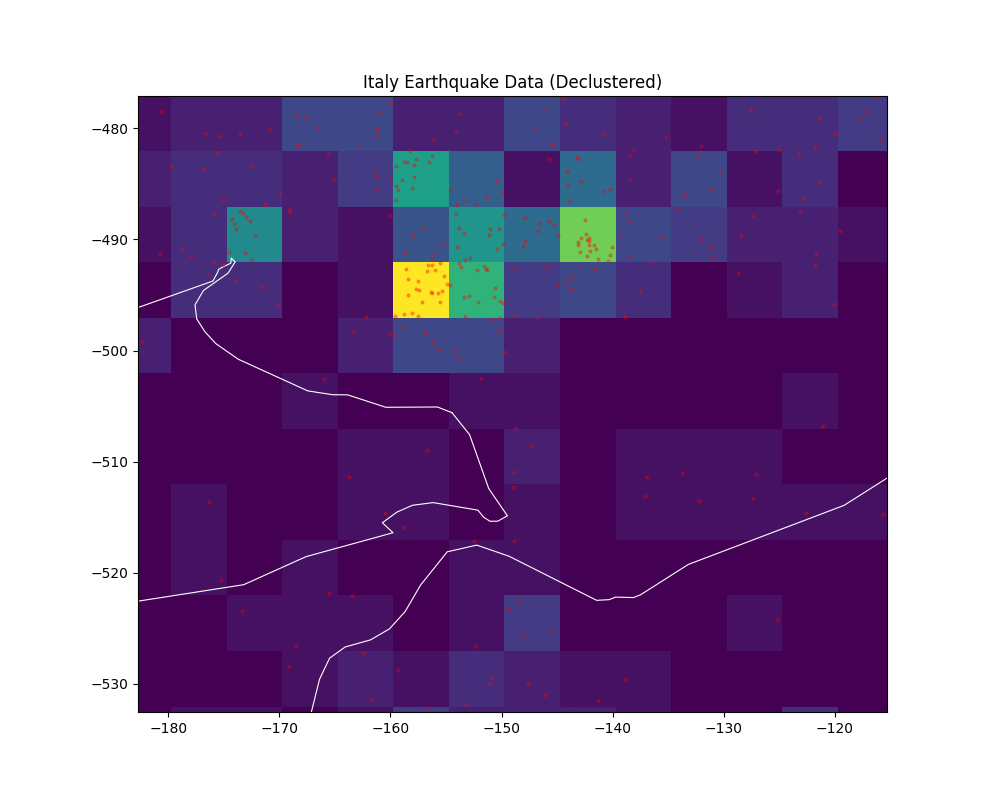
\includegraphics[width=\linewidth,height=0.70\textheight,keepaspectratio]{figures/italy_binned_zoom.png}

\column{0.34\textwidth}

\vspace{0.7cm}

$$\begin{gathered}
 n_i \mid f_i \sim \operatorname{Poisson}(\lambda_i)
\\[0.4cm]
f \sim \mathcal{N}(\mu,Q^{-1})
\\[0.4cm]
 \lambda_i = \lambda\,\sigmoid(f_i),
 \\[0.4cm]
 \sigmoid(f)=\frac{1}{1+e^{-f}}.
\end{gathered}$$





\end{columns}

 \end{frame}

% -----------------------------------------------------------
\begin{frame}{Bayesian spatial Poisson model}

\textbf{Likelihood}

\small
$$ n_i \mid f_i \sim \mathrm{Poi}\!\left(\lambda\,\sigma(f_i)\right),
\qquad
\sigma(f_i)=\frac{1}{1+e^{-f_i}}, $$
$$\mathcal{L}(f \mid n)=\prod_{i=1}^N \frac{(\lambda\sigma(f_i))^{n_i}}{n_i!} e^{-\lambda\sigma(f_i)}.$$


\textbf{Spatial prior}

$$f \sim \mathcal{N}(\mu,Q^{-1}),$$

\textbf{Posterior}

$$\log \mathbb{P}(f\mid n)
= \sum_{i=1}^N
\left(
n_i\log\{\lambda\sigma(f_i)\}
-\lambda\sigma(f_i)
\right)-\frac12(f-\mu)^\top Q(f-\mu)+c .$$


\begin{block}{The computational problem}
The posterior is not Gaussian, so we cannot directly sample from it.
\end{block}

\end{frame}

% -----------------------------------------------------------------------------------------
\begin{frame}{Sampling from the posterior}

$$\boxed{
\substack{
\text{Current field}\\
f^{(t)}
}}
\;\longrightarrow\;
\boxed{
\substack{
\text{Auxiliary counts}\\
k
}}
\;\longrightarrow\;
\boxed{
\substack{
\text{Pólya--Gamma}\\
\omega
}}
\;\longrightarrow\;
\boxed{
\substack{
\text{New field}\\
f^{(t+1)}
}}
$$

\vspace{0.6cm}


$$\begin{gathered}
k_i \sim \mathrm{Poisson}\!\left(\lambda\sigma(-f_i)\right)
\\[0.4cm]
\omega_i \sim \mathrm{PG}(n_i+k_i,f_i)
\\[0.4cm]
f\mid n,k,\omega \sim \mathcal{N}(m_{\mathrm{post}},Q_{\mathrm{post}}^{-1})
\end{gathered}$$

\end{frame}

% ---------------------------------------------------------------------
\begin{frame}{Conditional posterior after augmentation}

With the augmented variables \(k\) and \(\omega\), the latent field has a Gaussian conditional posterior


$$f \mid n,k,\omega
\sim
\mathcal N\!\left(m_{\mathrm{post}},\,Q_{\mathrm{post}}^{-1}\right).$$

\vspace{0.3cm}

\textbf{Posterior precision}


$$Q_{\mathrm{post}} = Q + \Omega,
\qquad
\Omega = \mathrm{diag}(\omega_1,\dots,\omega_N).$$

\vspace{0.3cm}

\textbf{Posterior mean}


$$m_{\mathrm{post}} = Q_{\mathrm{post}}^{-1} \left( Q\mu_0 + \kappa\right),$$

with

$$\kappa_i = \frac{1}{2}(n_i-k_i).$$

\vspace{0.4cm}

\begin{block}{Interpretation}
The prior contributes the spatial structure through \(Q\), and the data enter
through the augmented terms \(\kappa\) and \(\Omega\).
\end{block}

\end{frame}

% -----------------------------------------------------------


\begin{frame}{Synthetic experiment: bars setup}

\begin{columns}[T,onlytextwidth]

\column{0.49\textwidth}
\centering
\textbf{True intensity field}\par\medskip

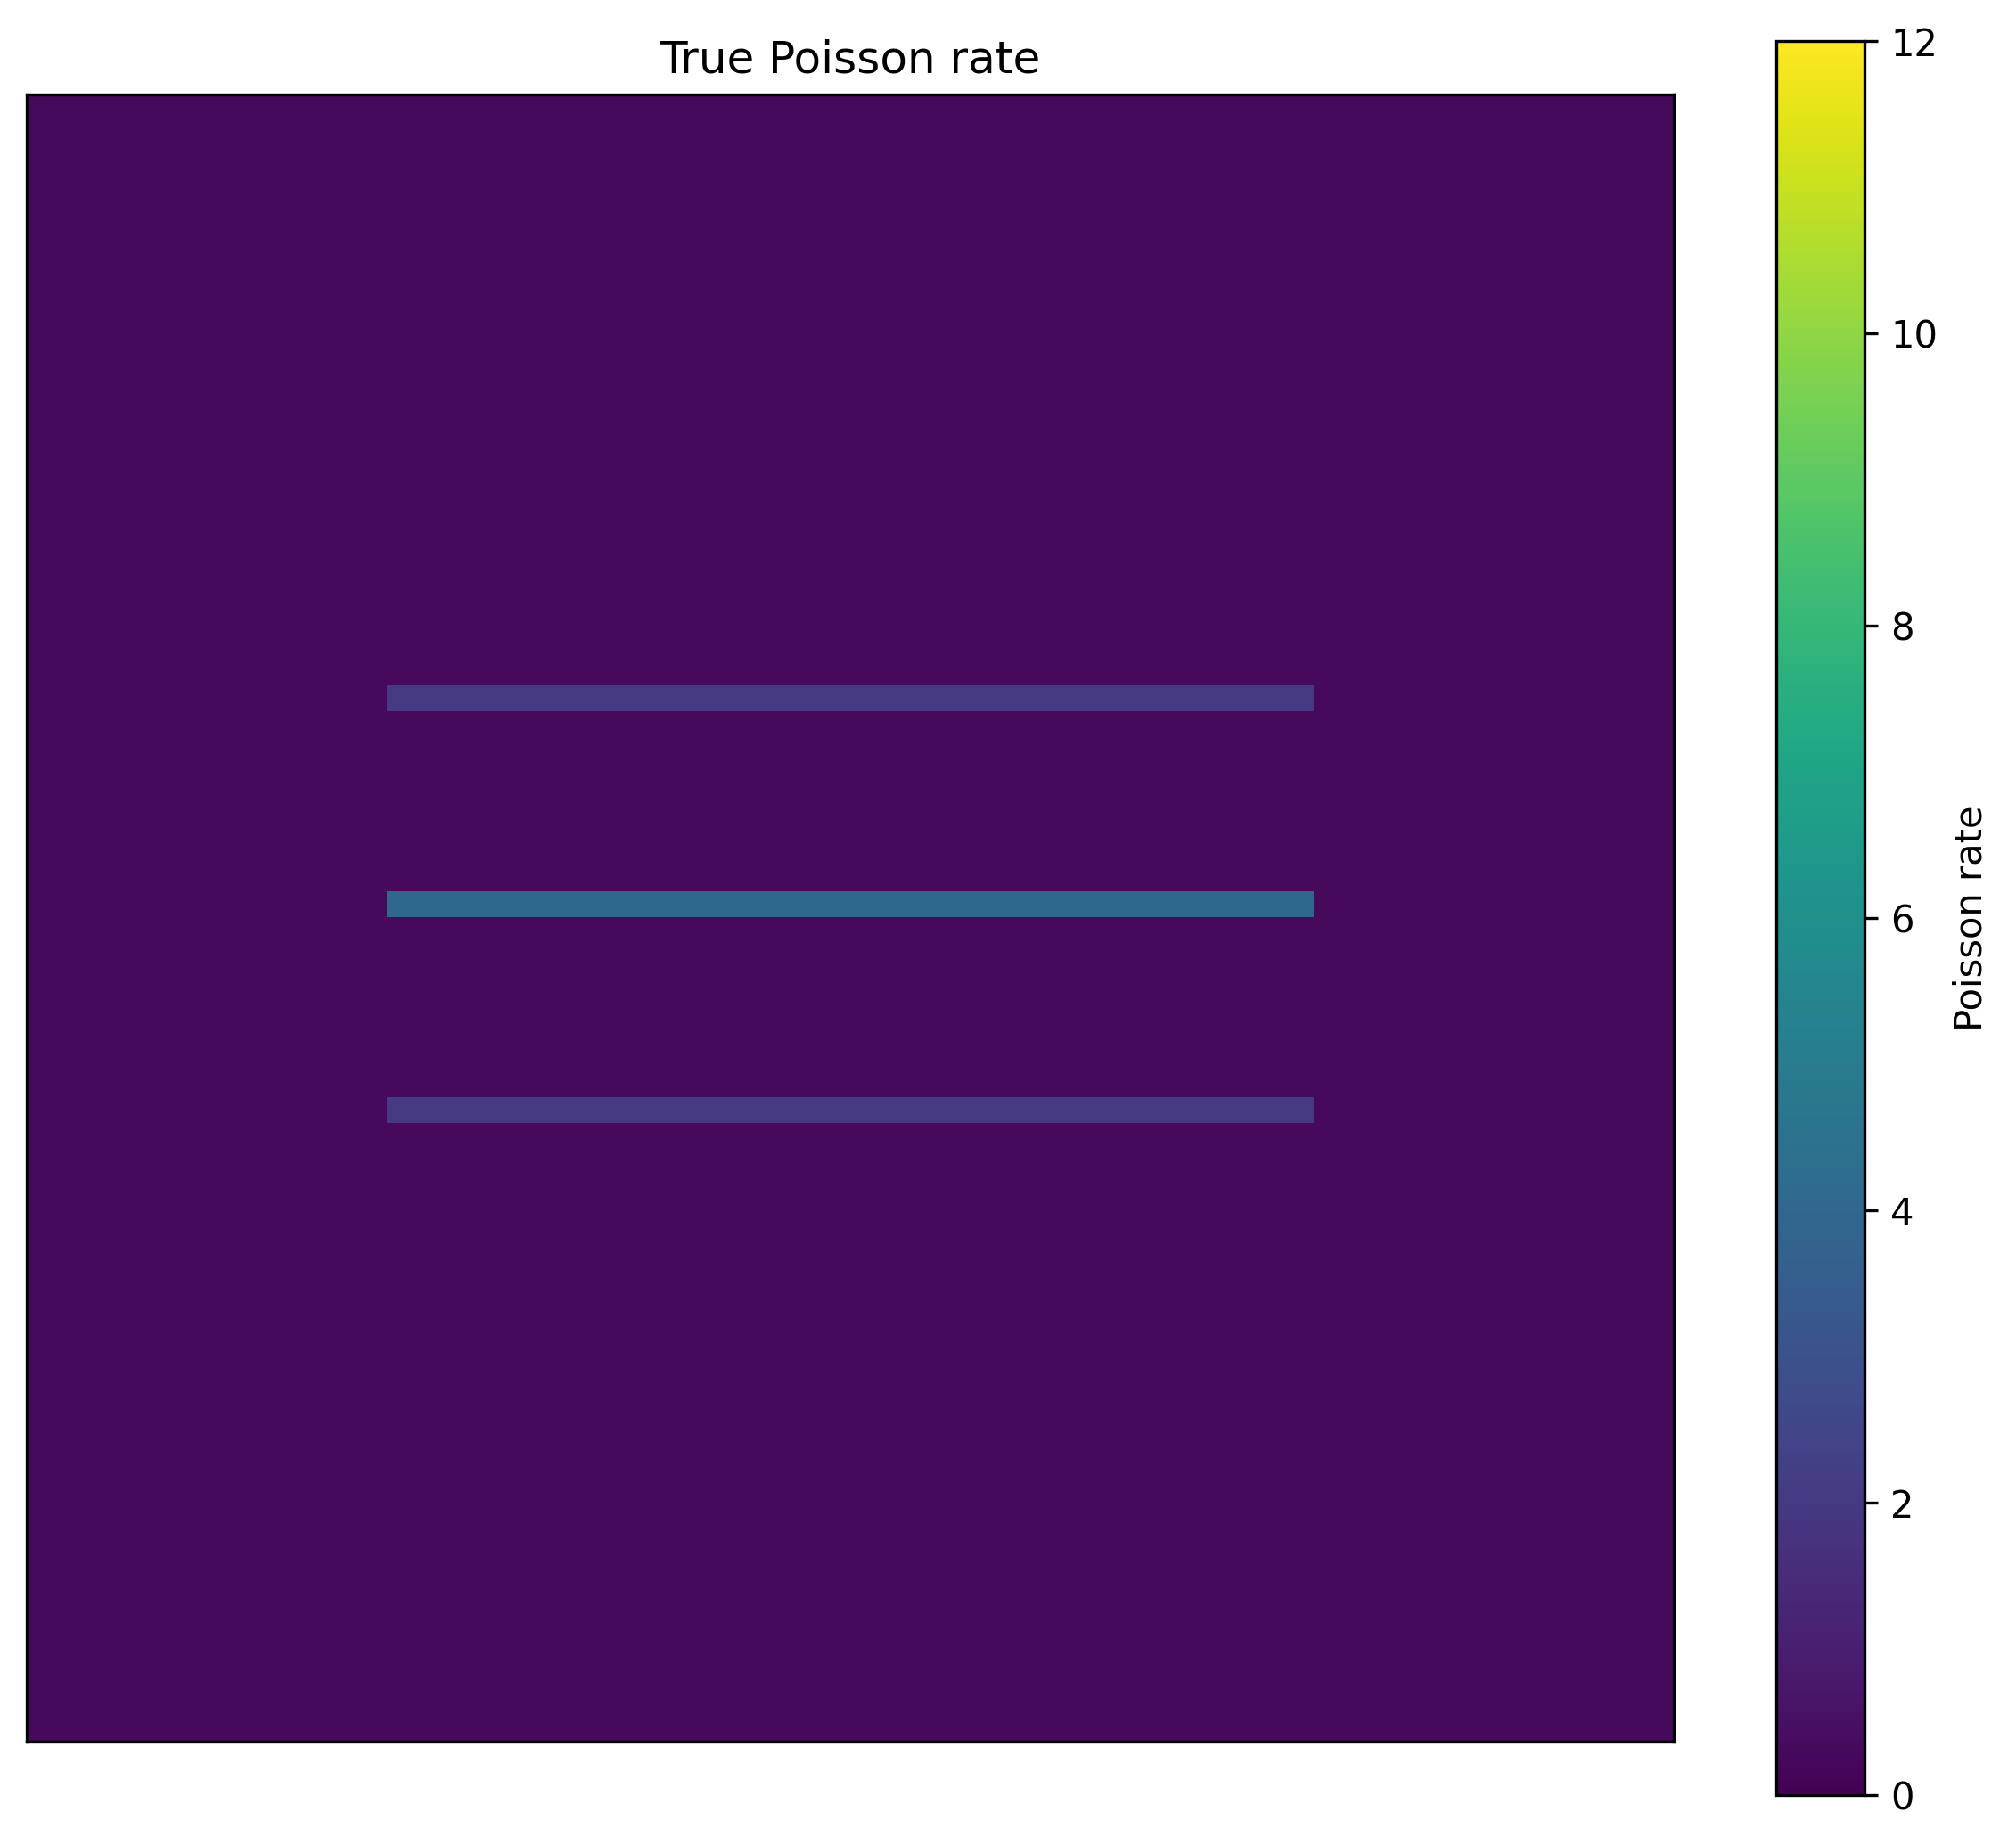
\includegraphics[
    width=\linewidth,
    height=0.45\textheight,
    keepaspectratio
]{figures/synthetic_bars_true_rate_rho_3_lam_12_var_4.png}


\column{0.49\textwidth}
\centering
\textbf{Observed Poisson counts}\par\medskip

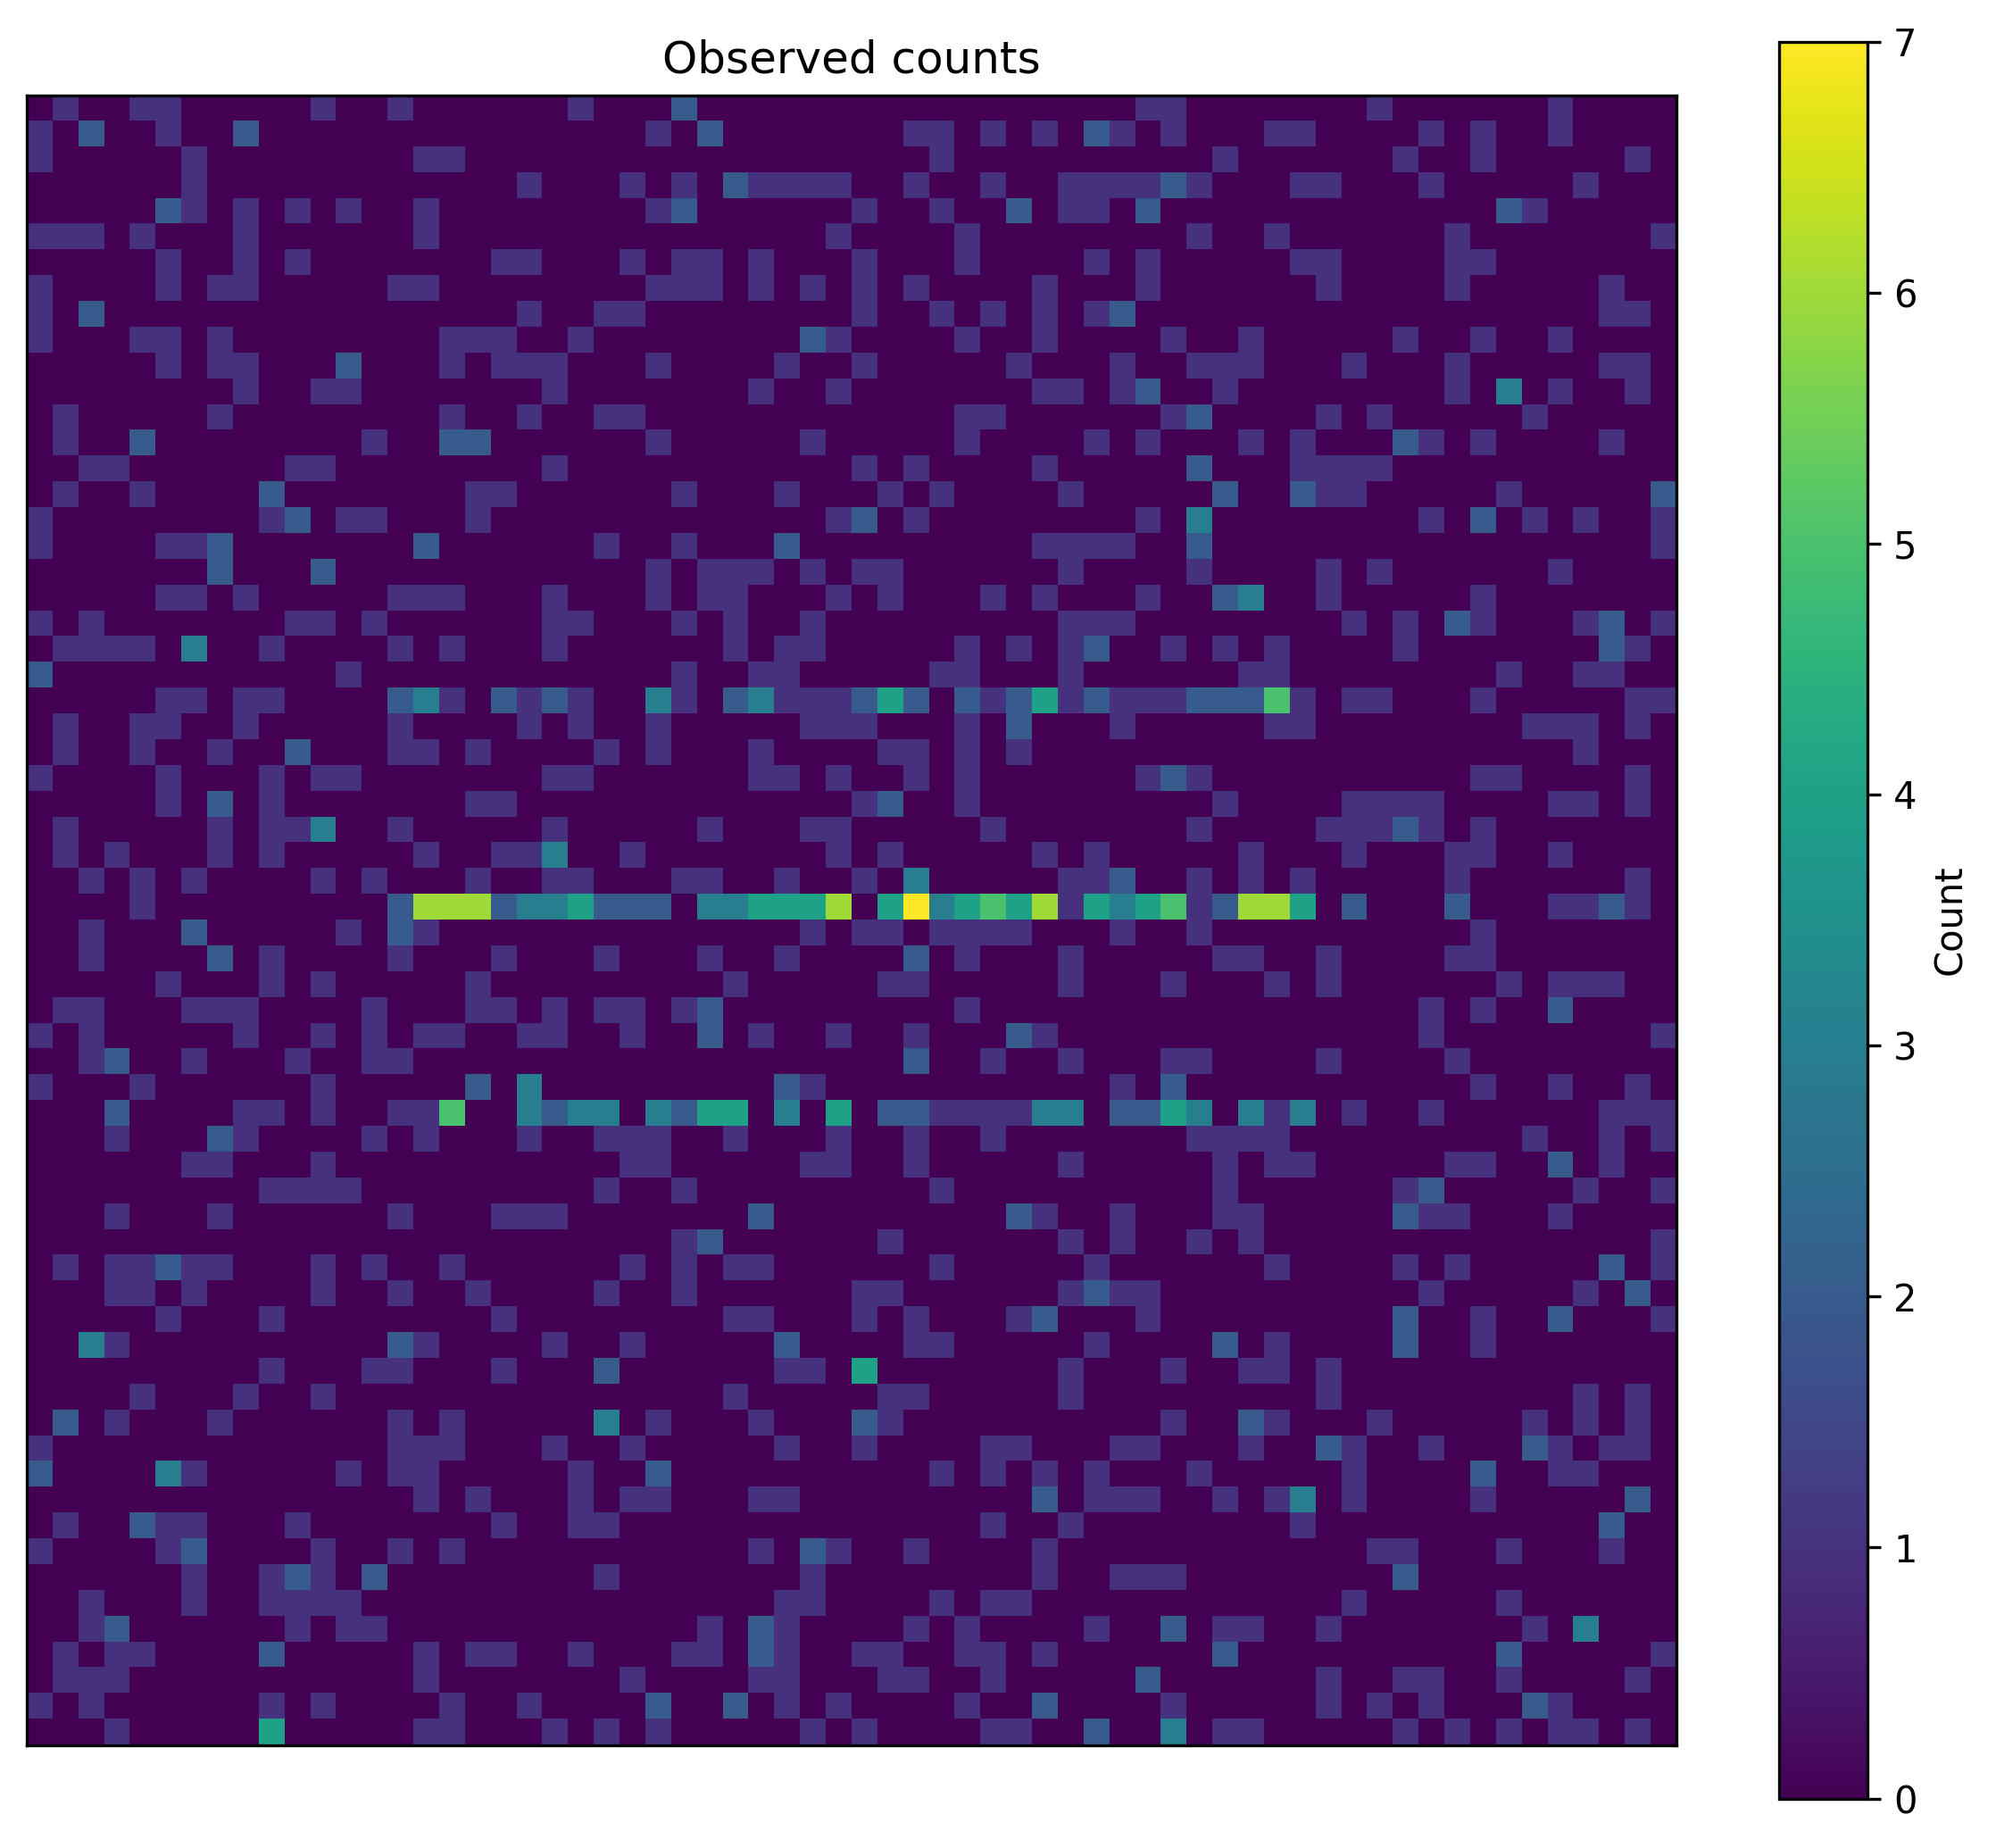
\includegraphics[
    width=\linewidth,
    height=0.45\textheight,
    keepaspectratio
]{figures/synthetic_bars_observed_counts_rho_3_lam_12_var_4.png}

\end{columns}

\vspace{0.25cm}

\small
\textbf{Purpose:}
Check whether the inference recovers elongated high-rate structures
from noisy count data.

\vspace{0.35cm}



\end{frame}


%--------------------------------------------
\begin{frame}{Synthetic experiment: bars inference}

\begin{columns}[T,onlytextwidth]

\column{0.5\textwidth}

\centering
\textbf{Posterior rate mean}\par\medskip

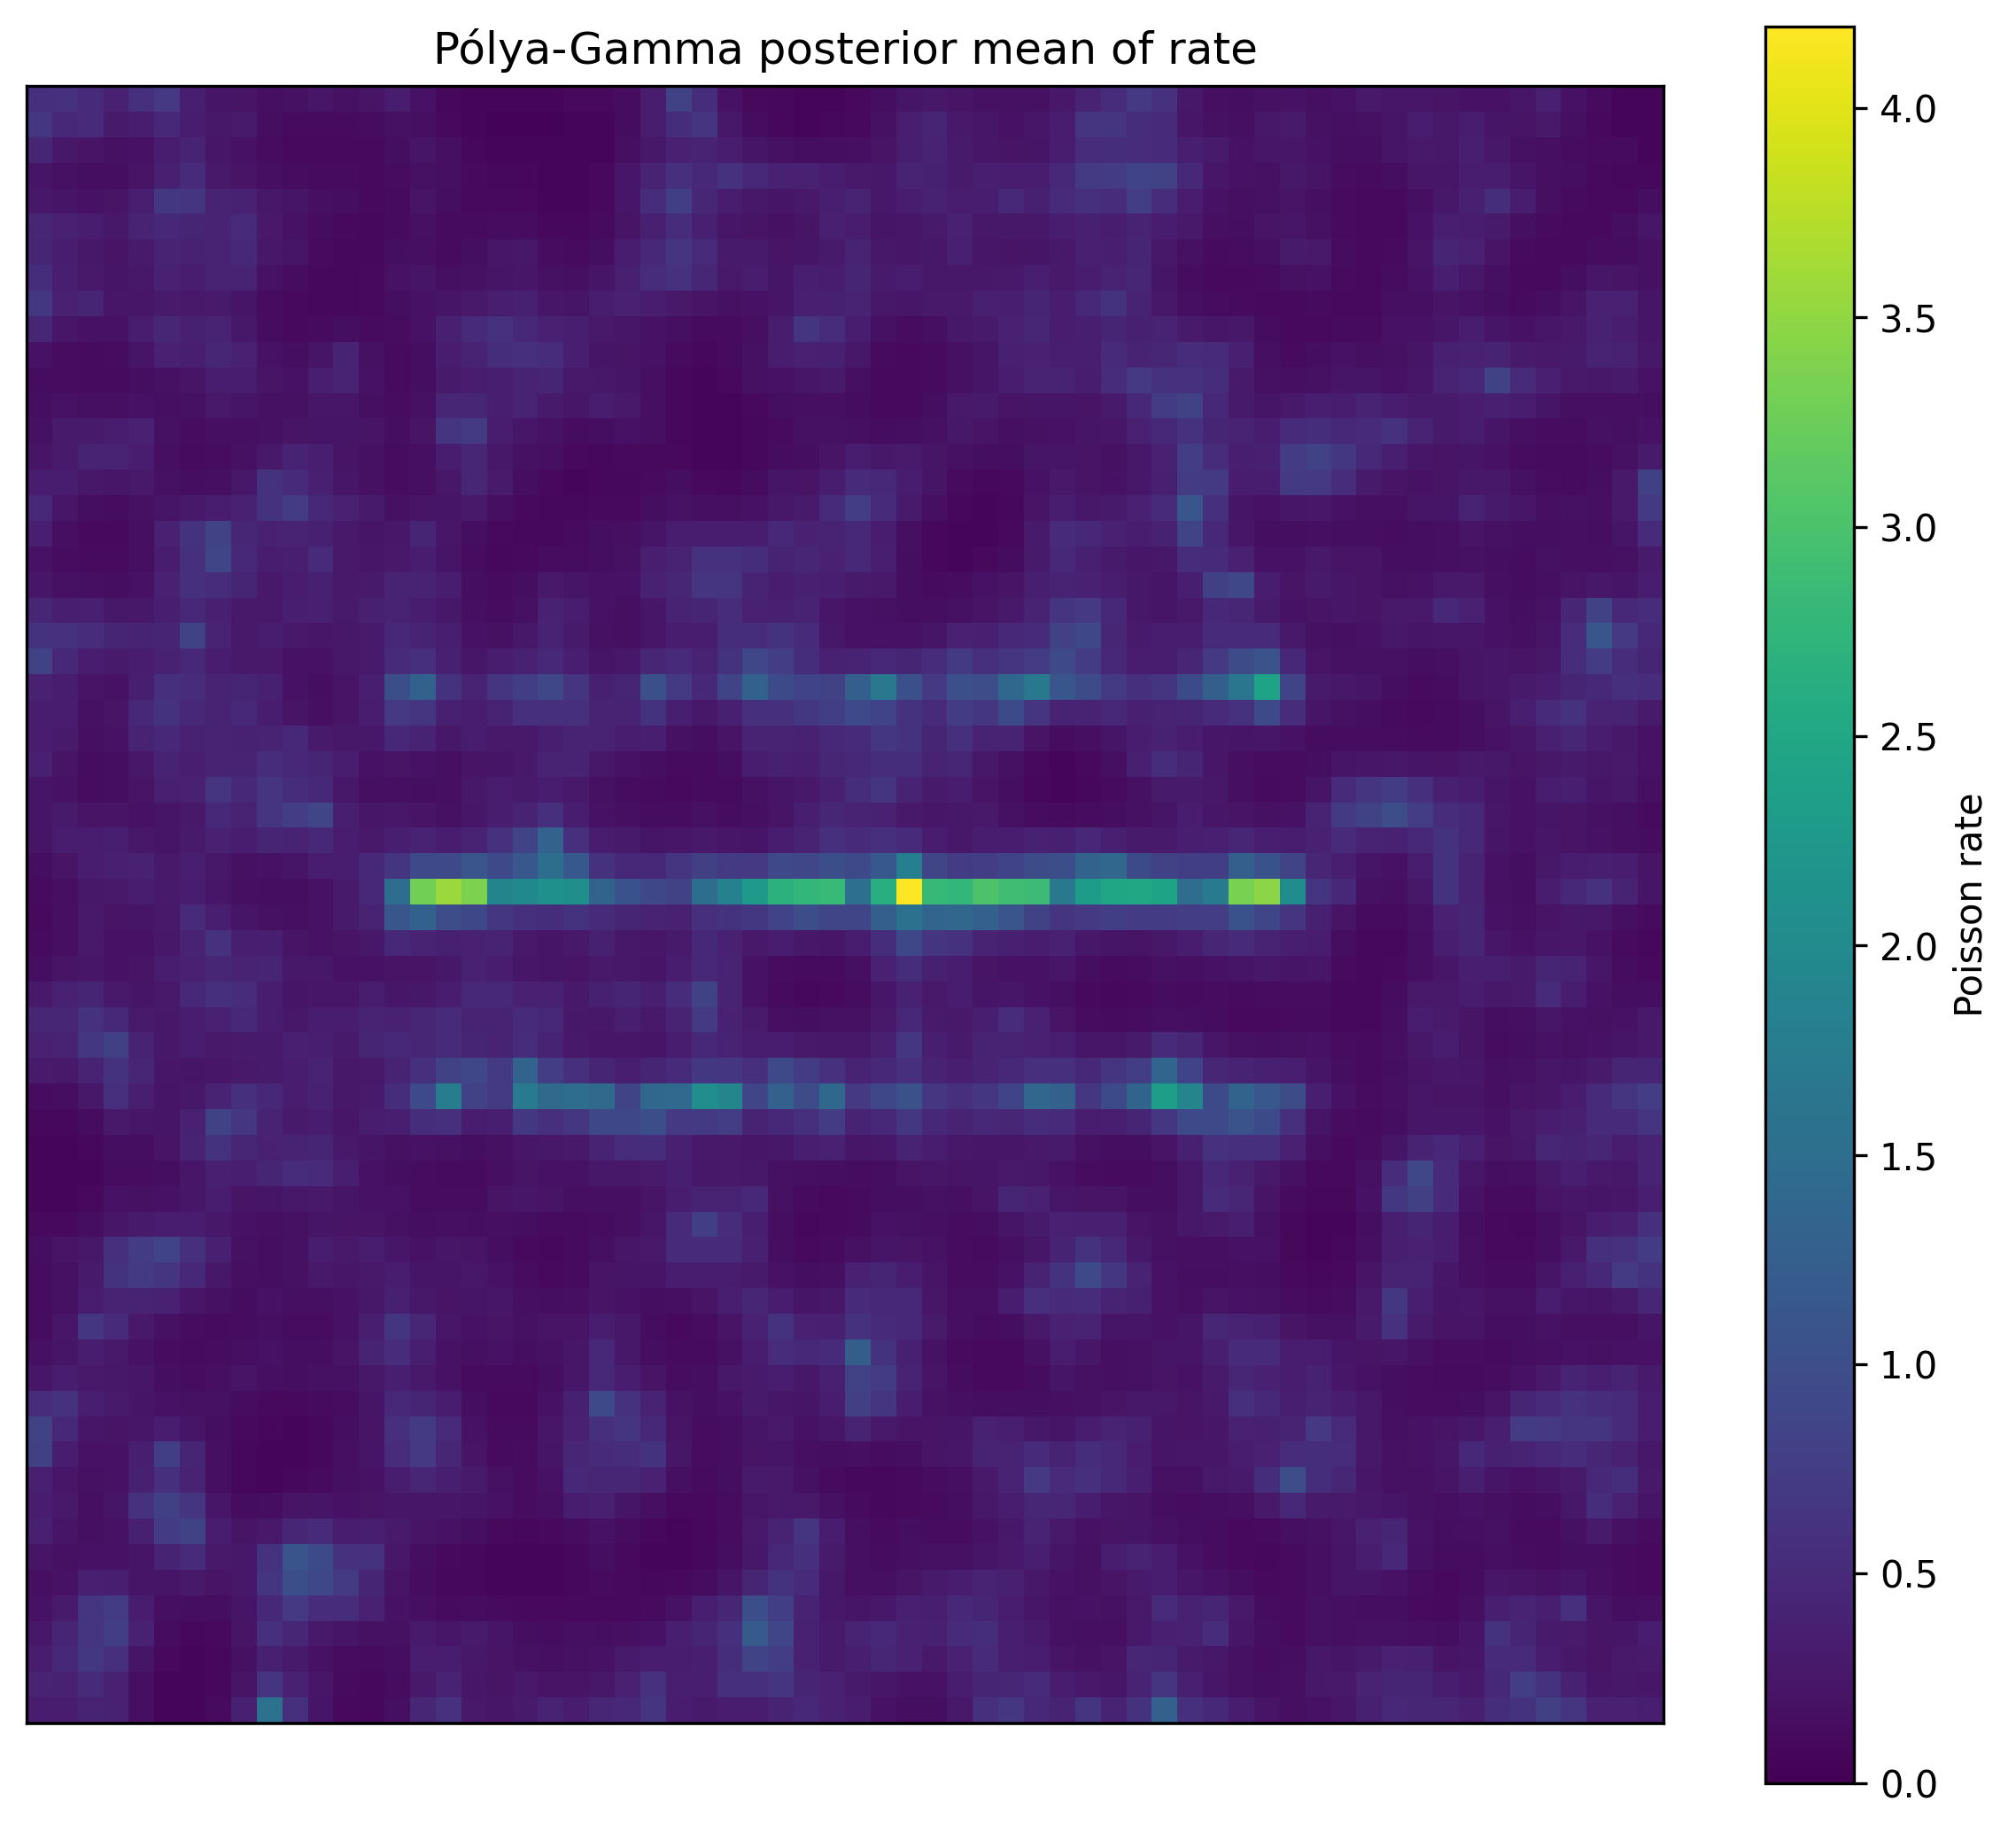
\includegraphics[
    width=\linewidth,
    height=\textheight,
    keepaspectratio
]{figures/synthetic_bars_posterior_mean_rate_rho_3_lam_12_var_4.png}







\column{0.50\textwidth}

\centering
\textbf{Posterior mean - MAP estimate}\par\medskip

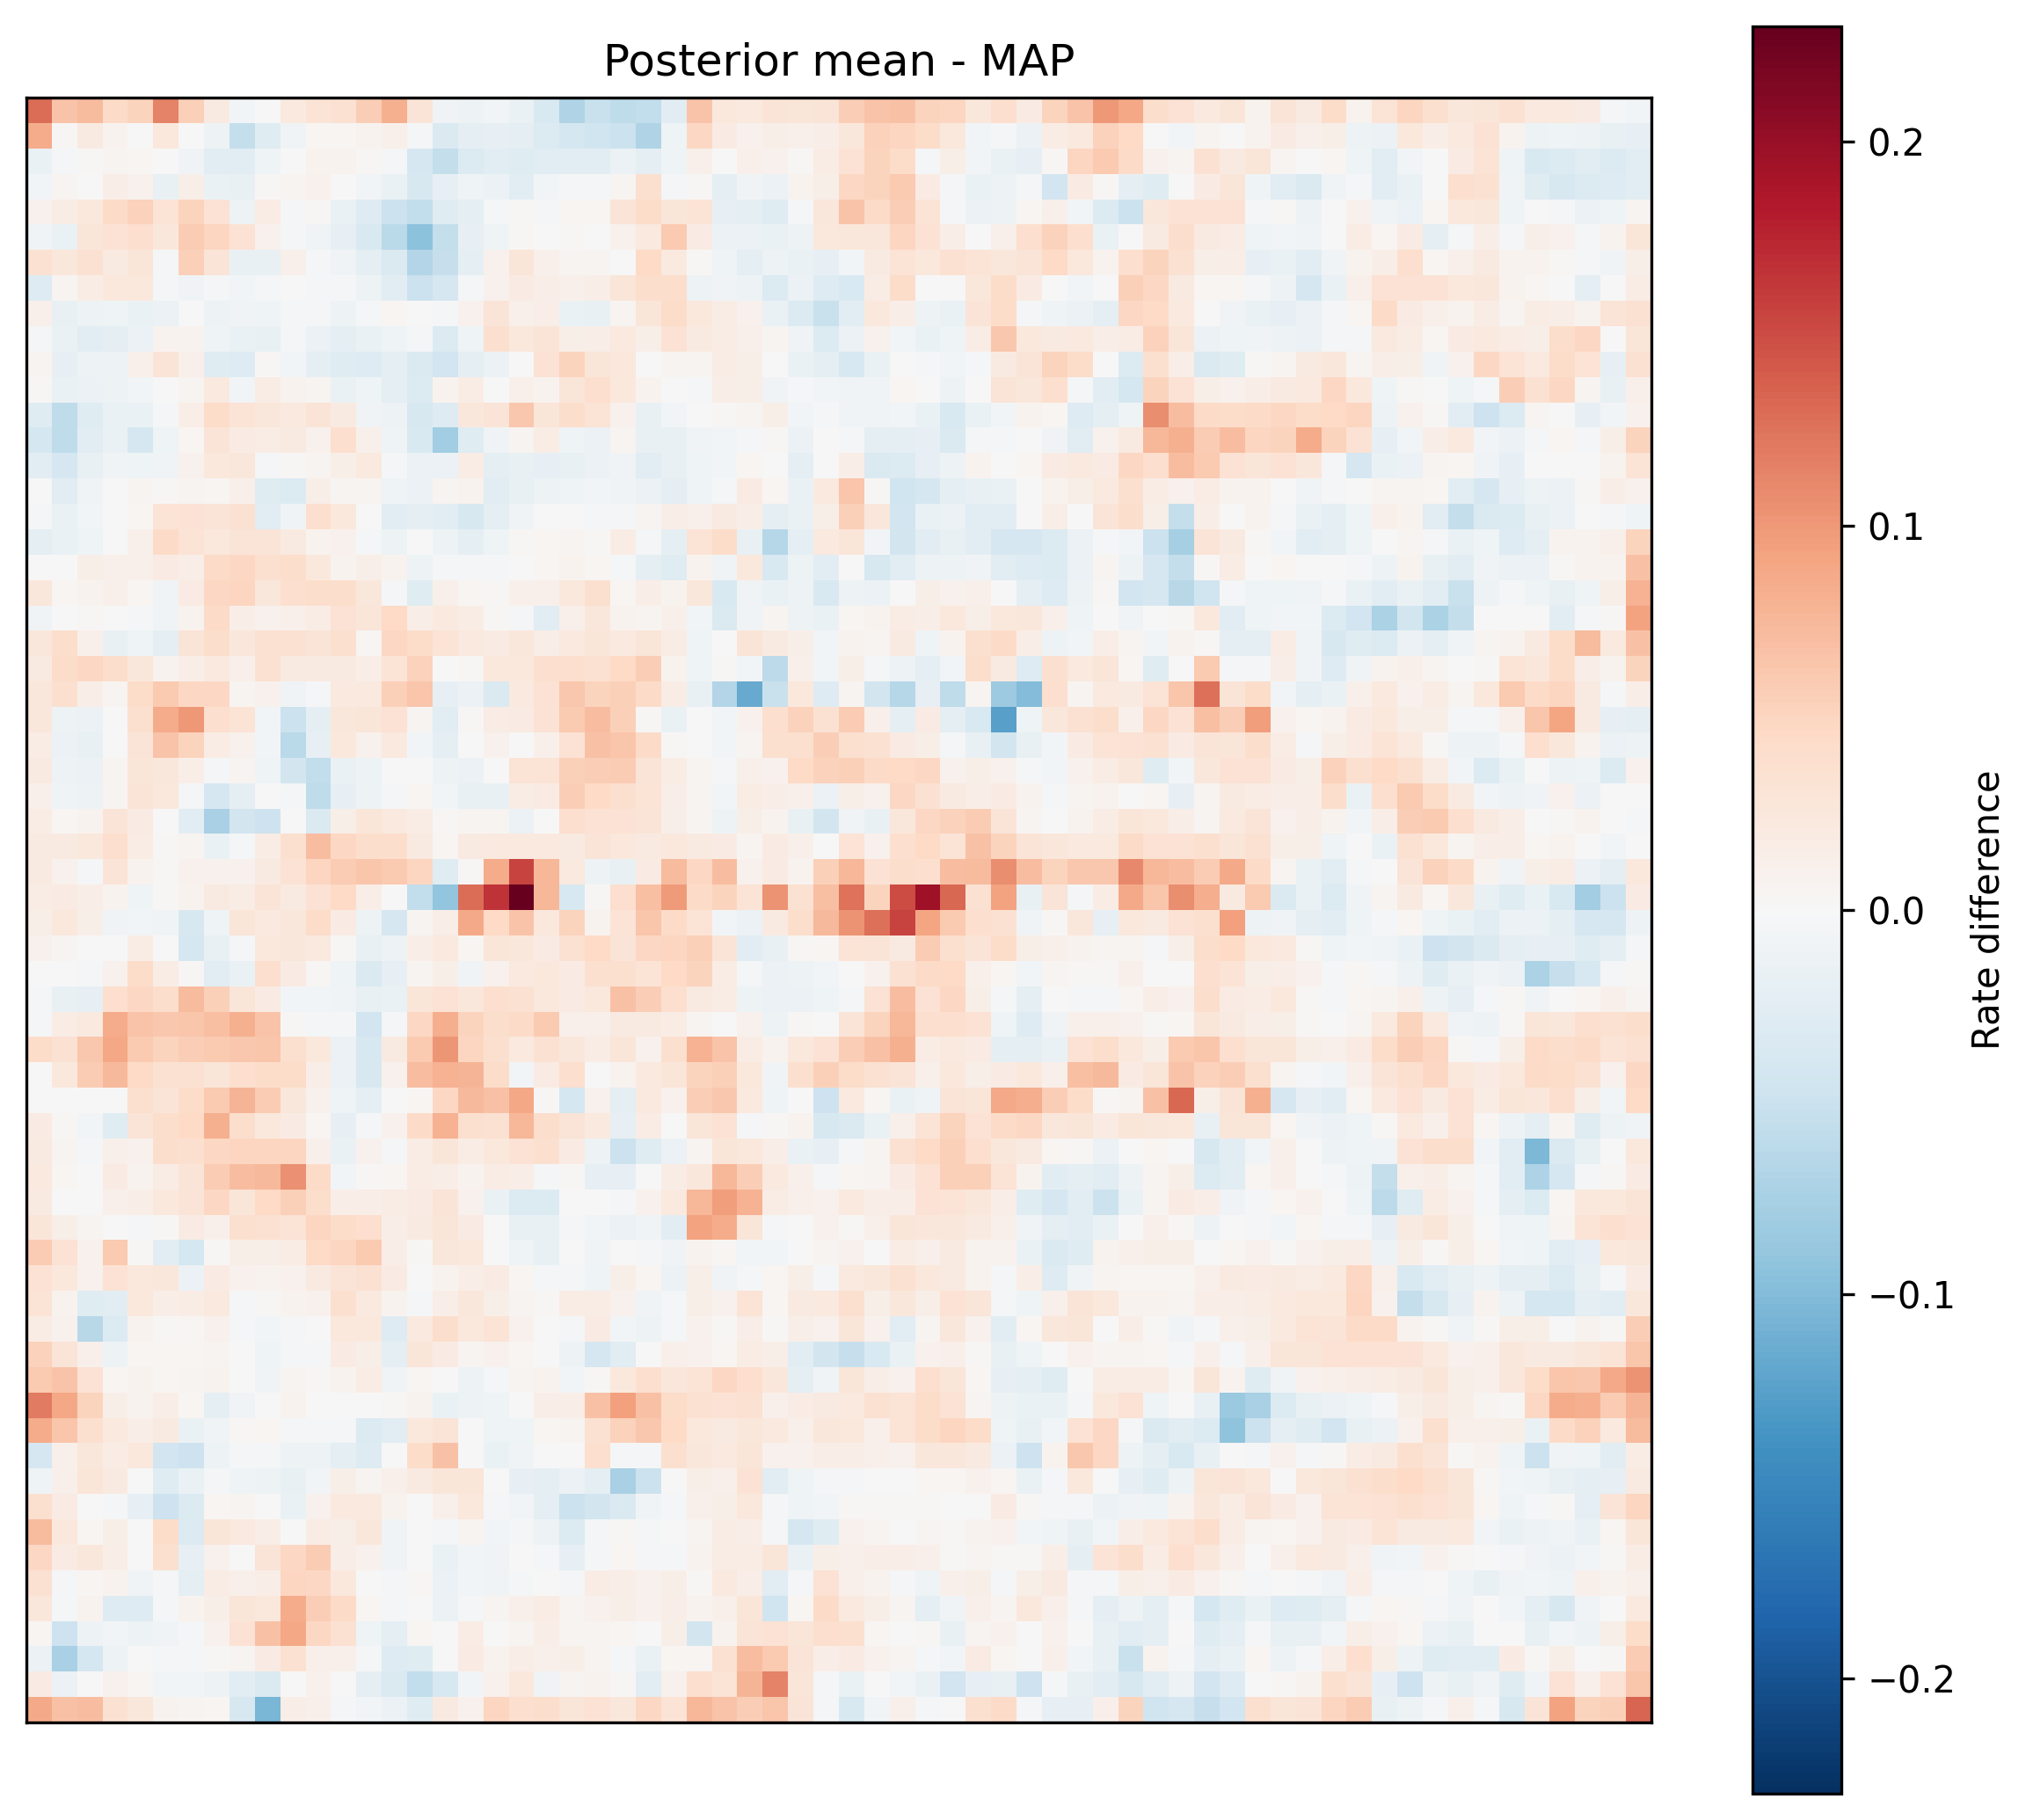
\includegraphics[
    width=\linewidth,
    height=\textheight,
    keepaspectratio
]{figures/synthetic_bars_posterior_mean_minus_map_rho_3_lam_12_var_4.png}

\end{columns}

\end{frame}


% ---------------------------
\begin{frame}{Synthetic experiment}
\centering
    \textbf{Posterior samples}\par\medskip

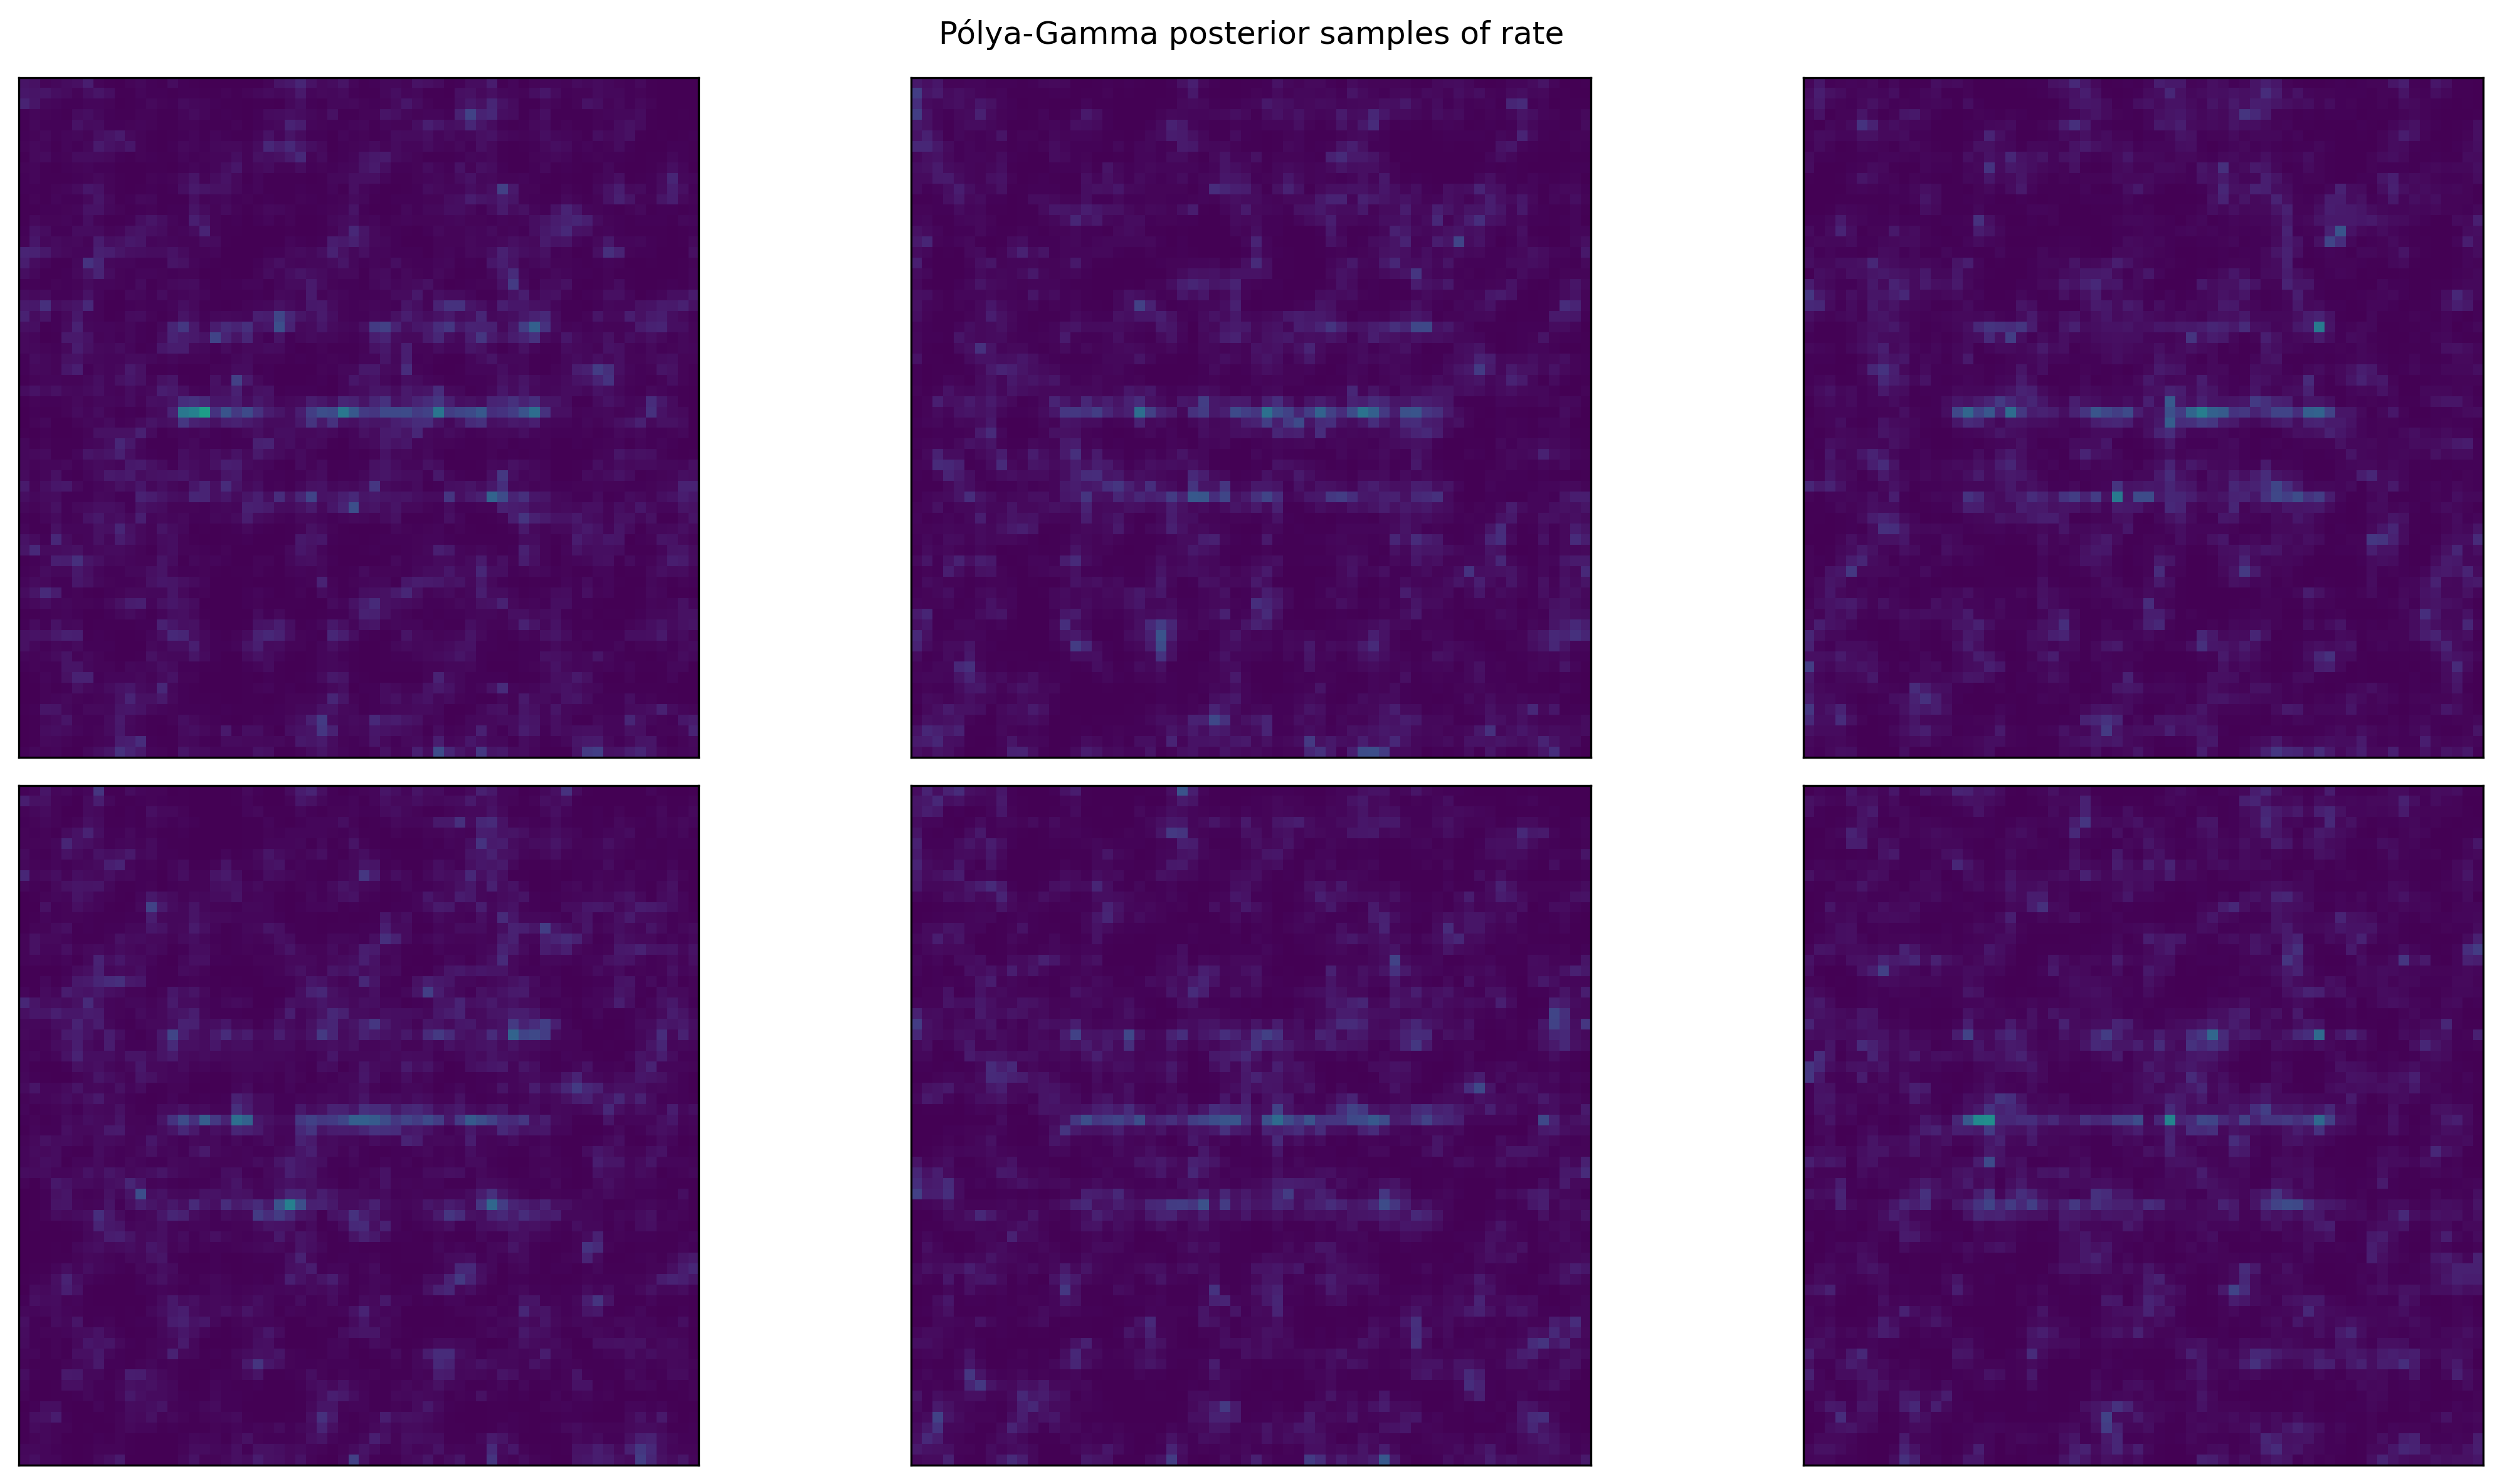
\includegraphics[
    width=\linewidth,
    height=0.66\textheight,
    keepaspectratio
]{figures/synthetic_bars_posterior_samples_rho_3_lam_12_var_4.png}
\end{frame}

%---------------------------------------

\begin{frame}{Synthetic experiment: block setup}

\begin{columns}[T,onlytextwidth]

\column{0.49\textwidth}
\centering
\textbf{True intensity field}\par\medskip

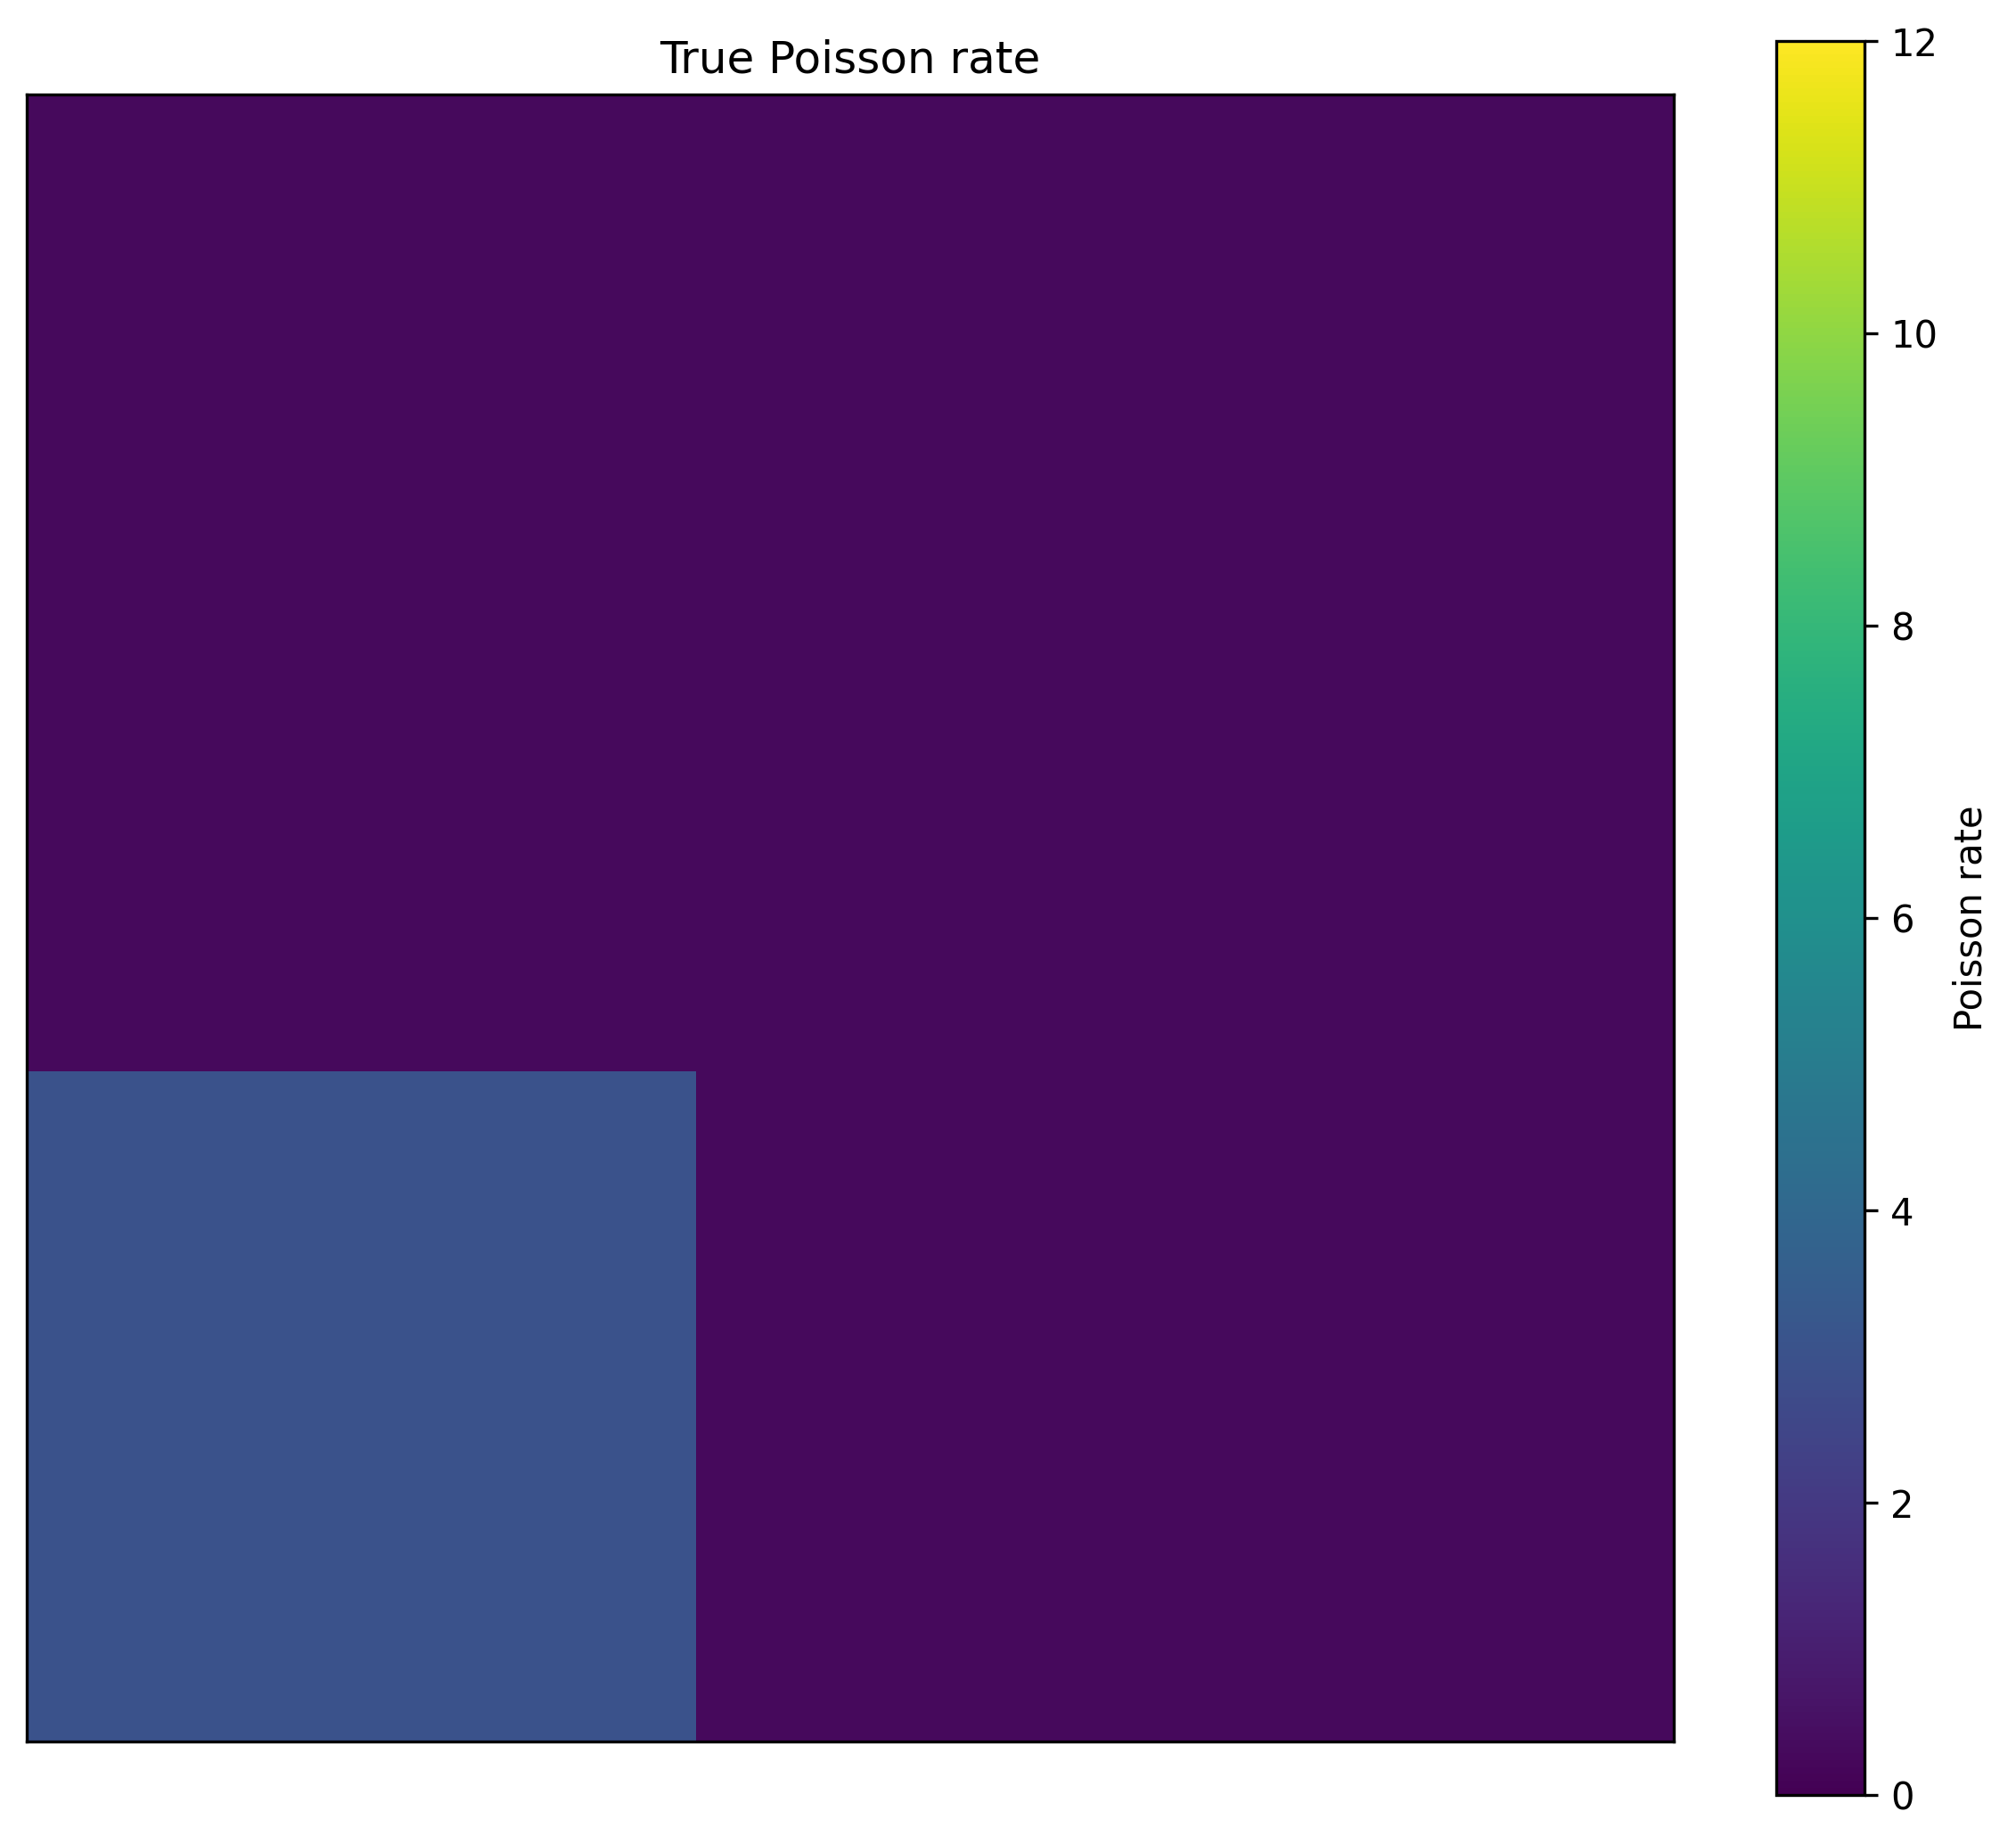
\includegraphics[
    width=\linewidth,
    height=0.45\textheight,
    keepaspectratio
]{figures/synthetic_block_true_rate_rho_2_lam_12_var_4.png}


\column{0.49\textwidth}
\centering
\textbf{Observed Poisson counts}\par\medskip

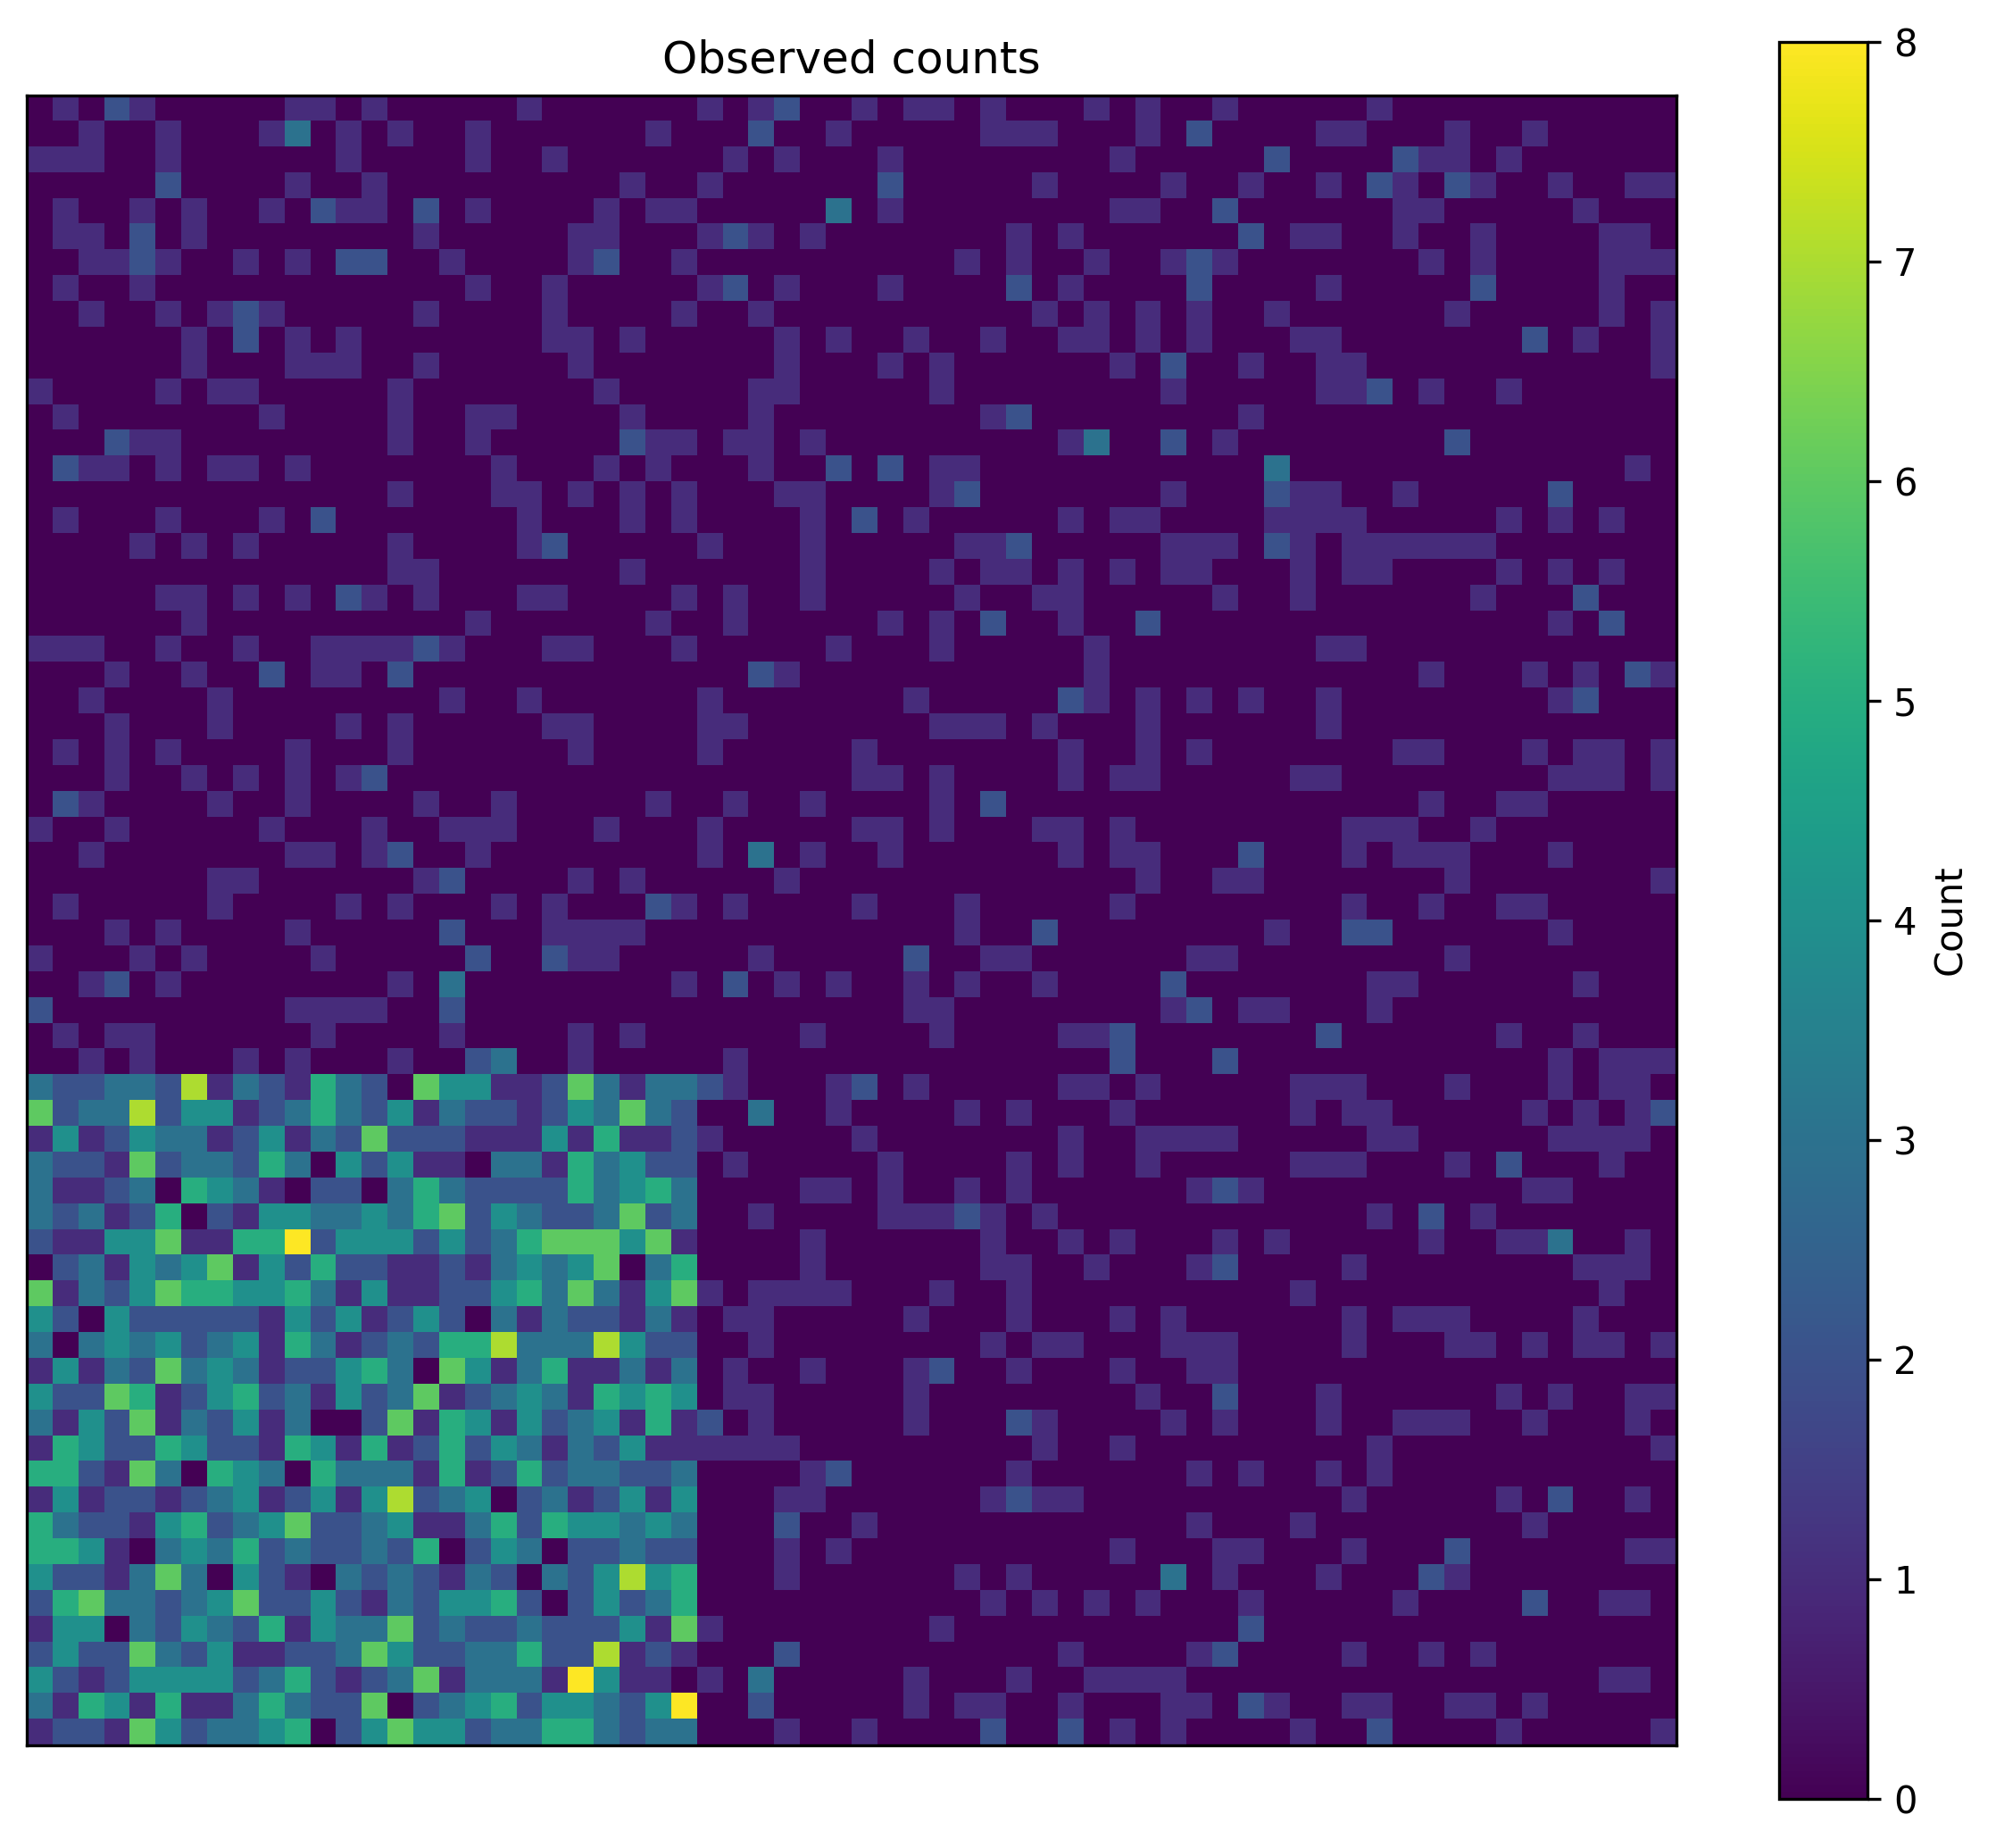
\includegraphics[
    width=\linewidth,
    height=0.45\textheight,
    keepaspectratio
]{figures/synthetic_block_observed_counts_rho_2_lam_12_var_4.png}

\end{columns}

\vspace{0.25cm}

\small
\textbf{Purpose:}
Check whether the inference recovers a compact high-rate region
while preserving the spatial contrast.

\vspace{0.35cm}



\end{frame}


% -----------------------------------------------------------
\begin{frame}{Synthetic experiment: block inference}

\begin{columns}[T,onlytextwidth]

\column{0.48\textwidth}

\centering
\textbf{Posterior mean}\par\medskip

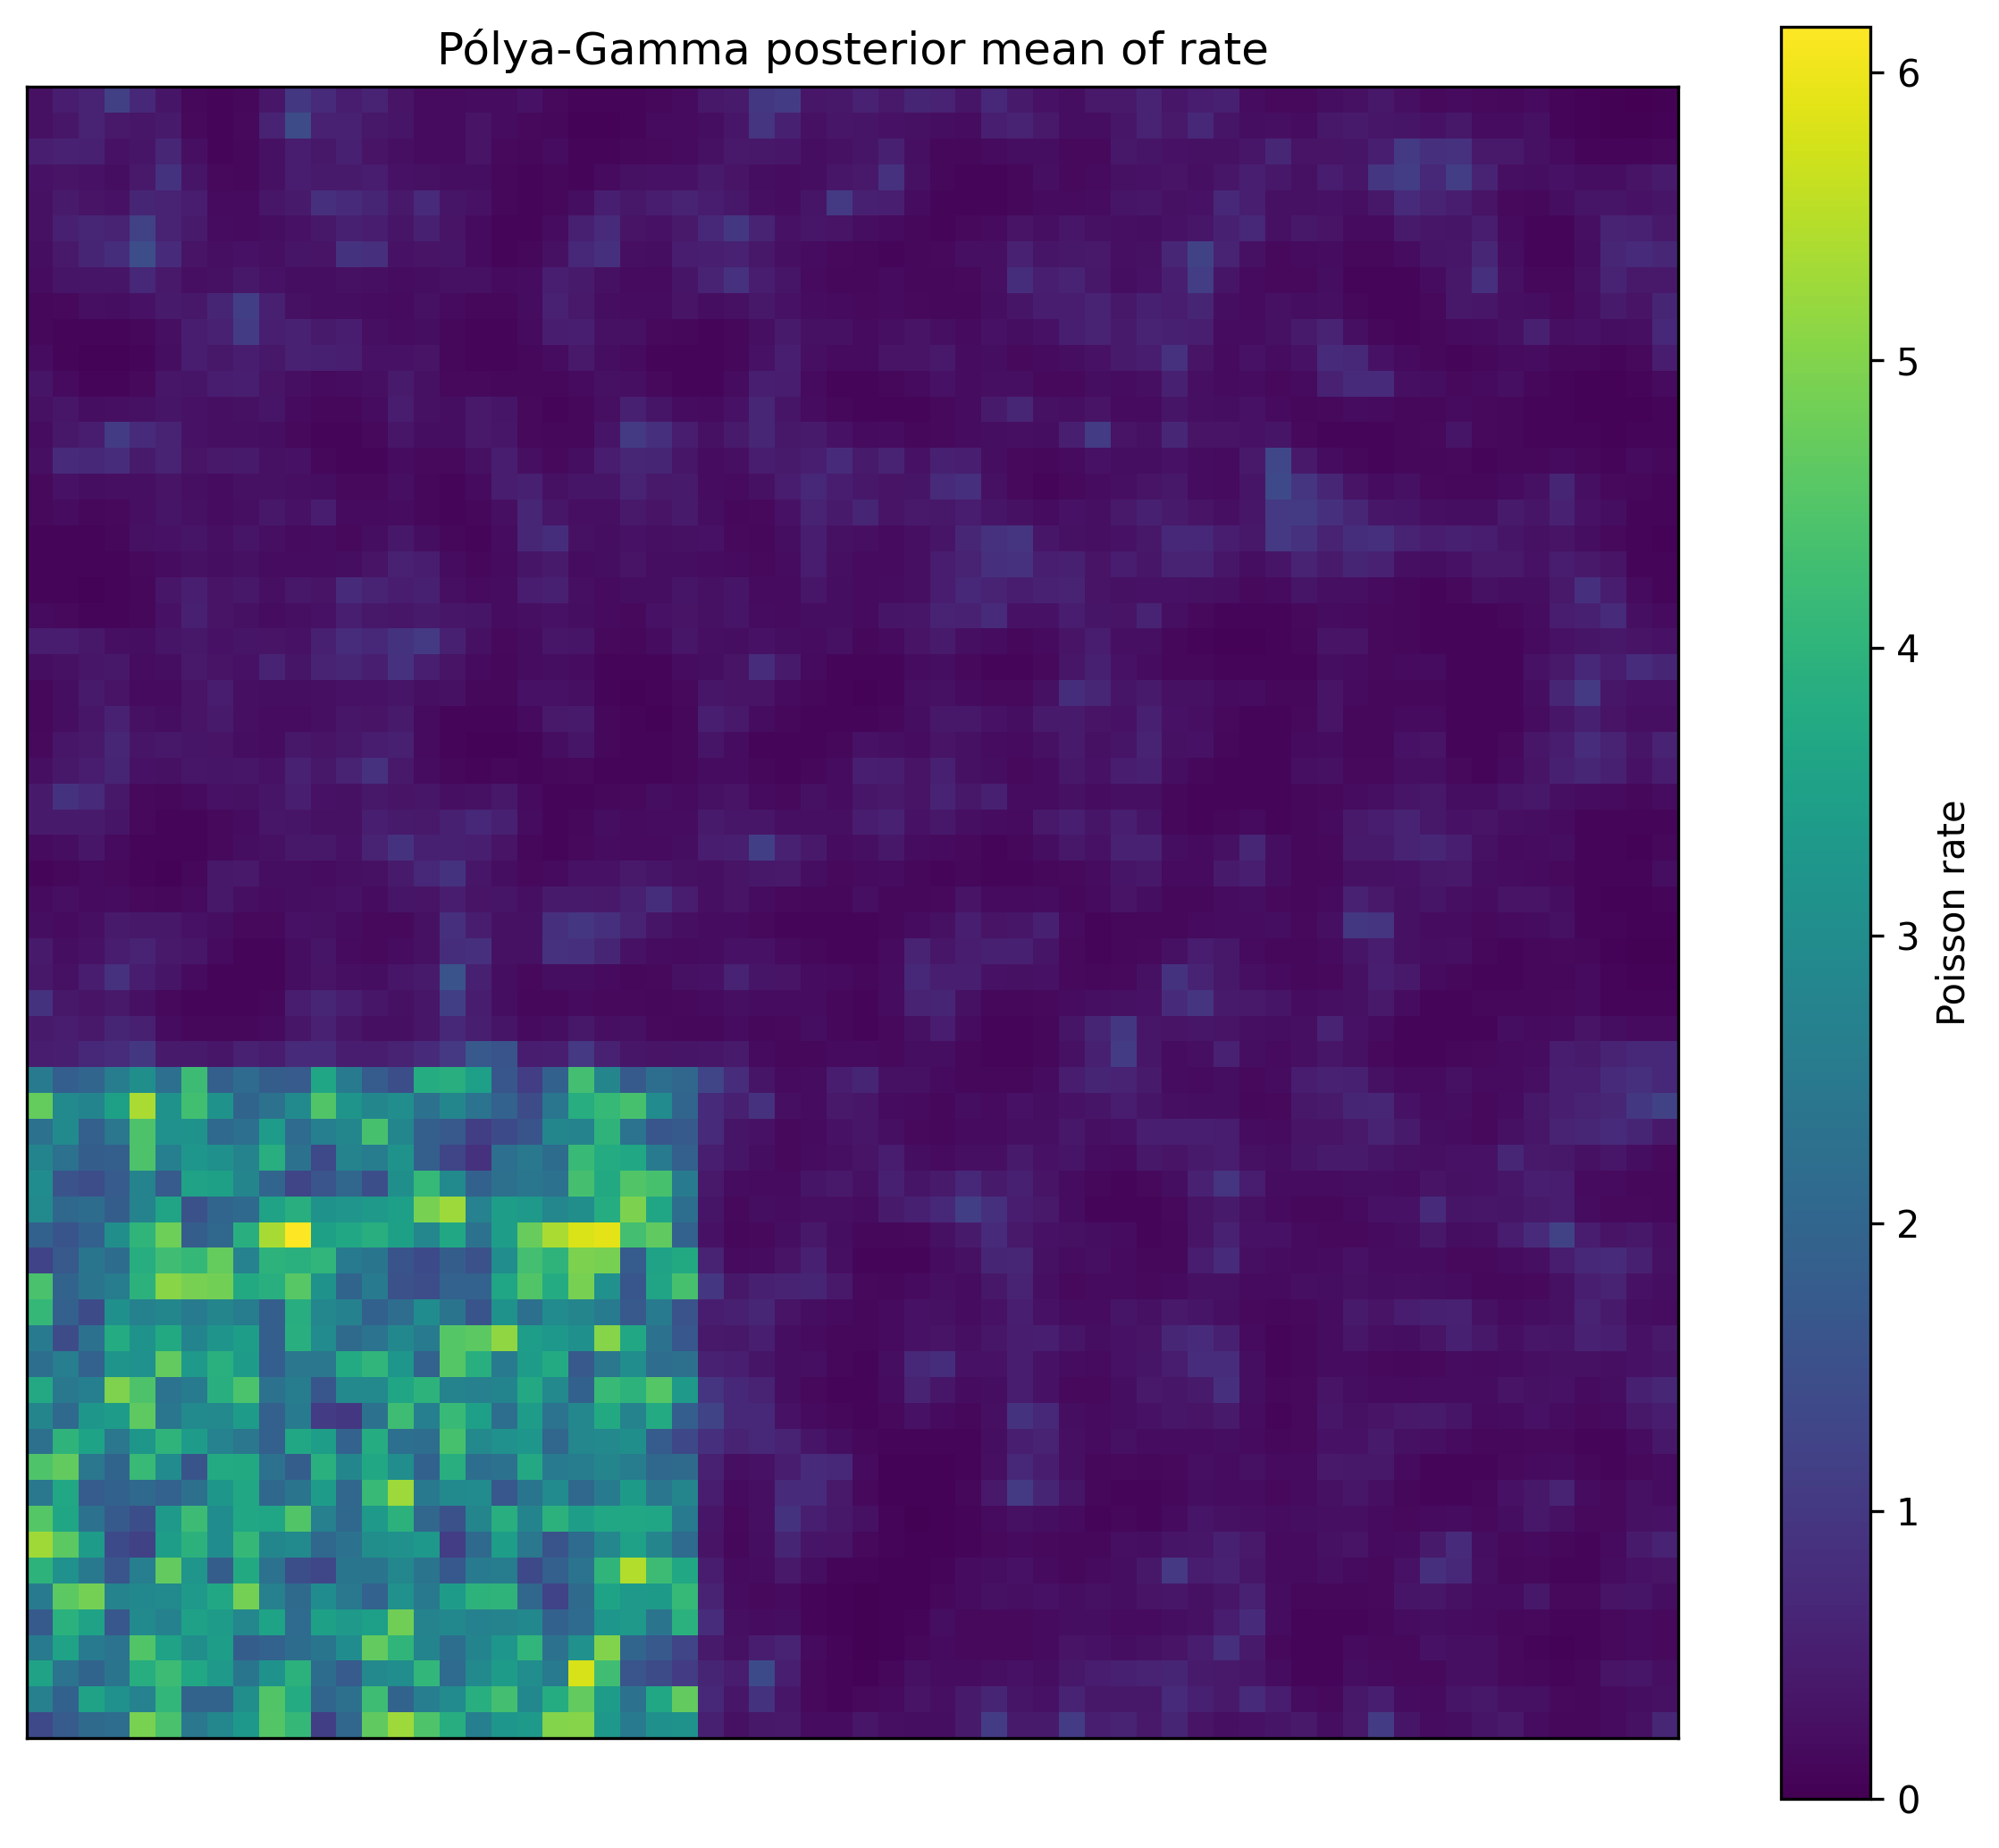
\includegraphics[
    width=\linewidth,
    height=\textheight,
    keepaspectratio
]{figures/synthetic_block_posterior_mean_rate_rho_2_lam_12_var_4.png}




\column{0.50\textwidth}

\centering
\textbf{Posterior mean - MAP estimate}\par\medskip

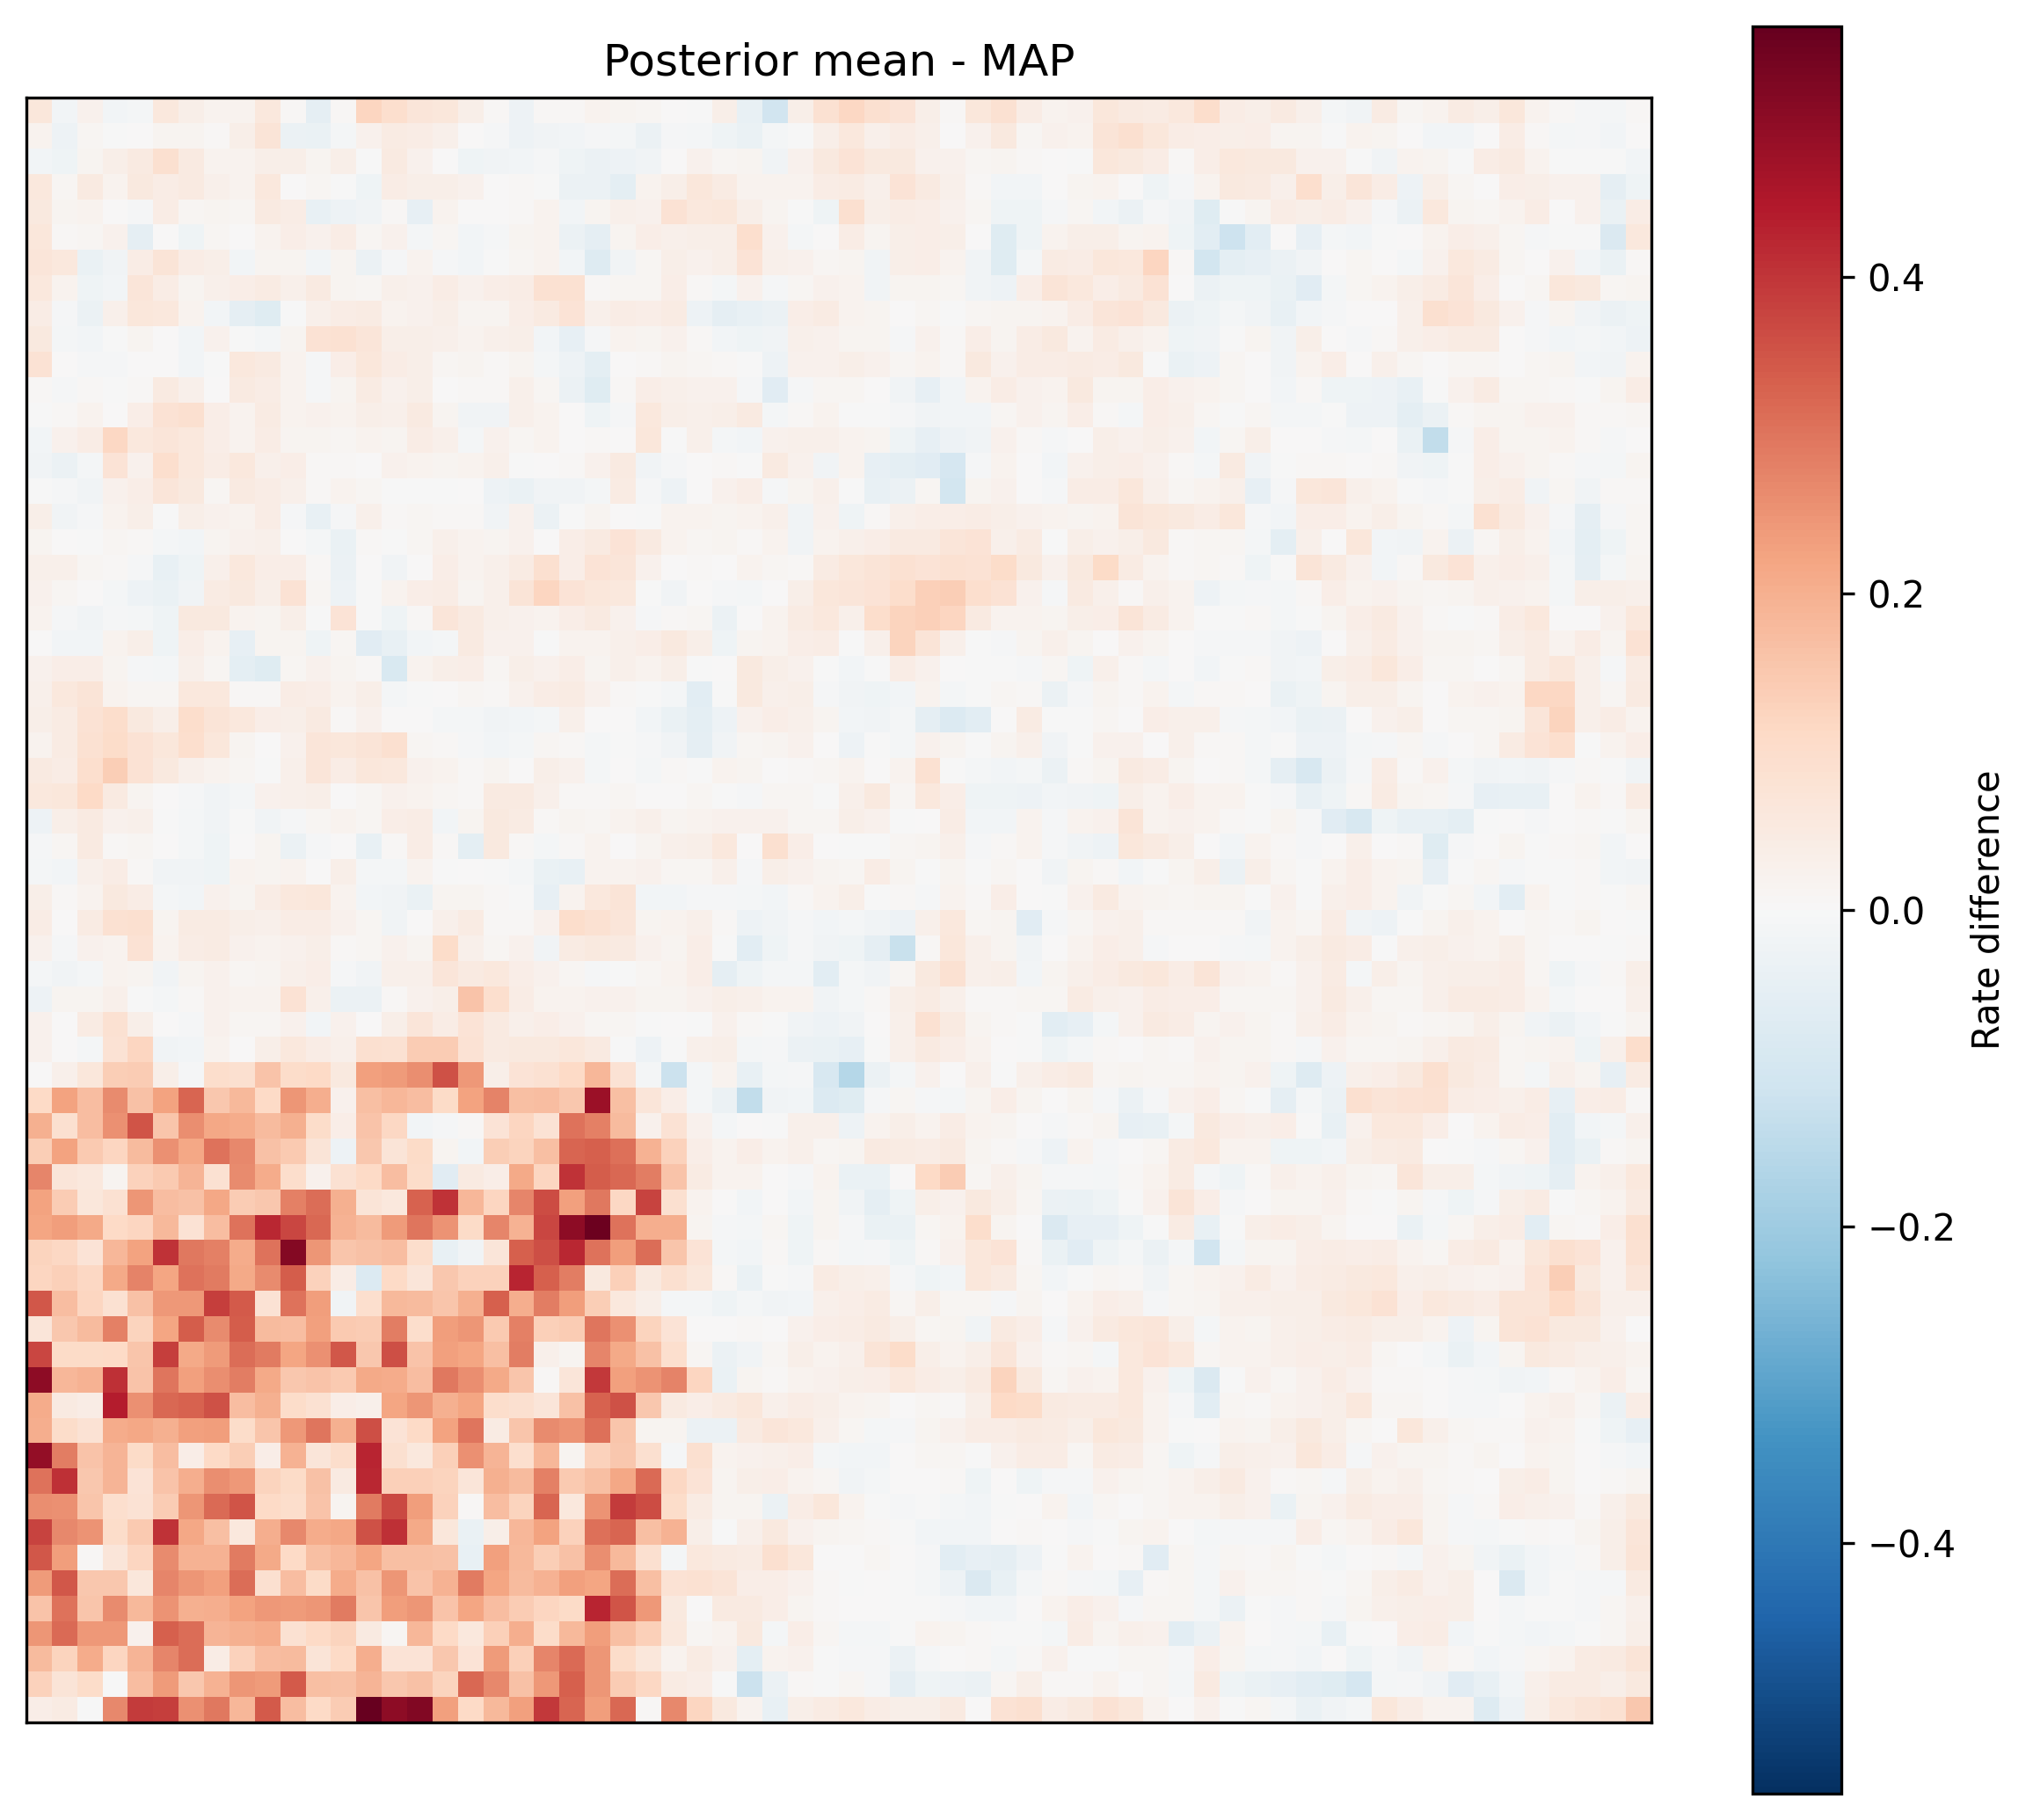
\includegraphics[
    width=\linewidth,
    height=\textheight,
    keepaspectratio
]{figures/synthetic_block_posterior_mean_minus_map_rho_2_lam_12_var_4.png}

\end{columns}

\end{frame}

%--------------------------------
\begin{frame}{Synthetic experiment}
   \centering
\textbf{Posterior samples}\par\medskip

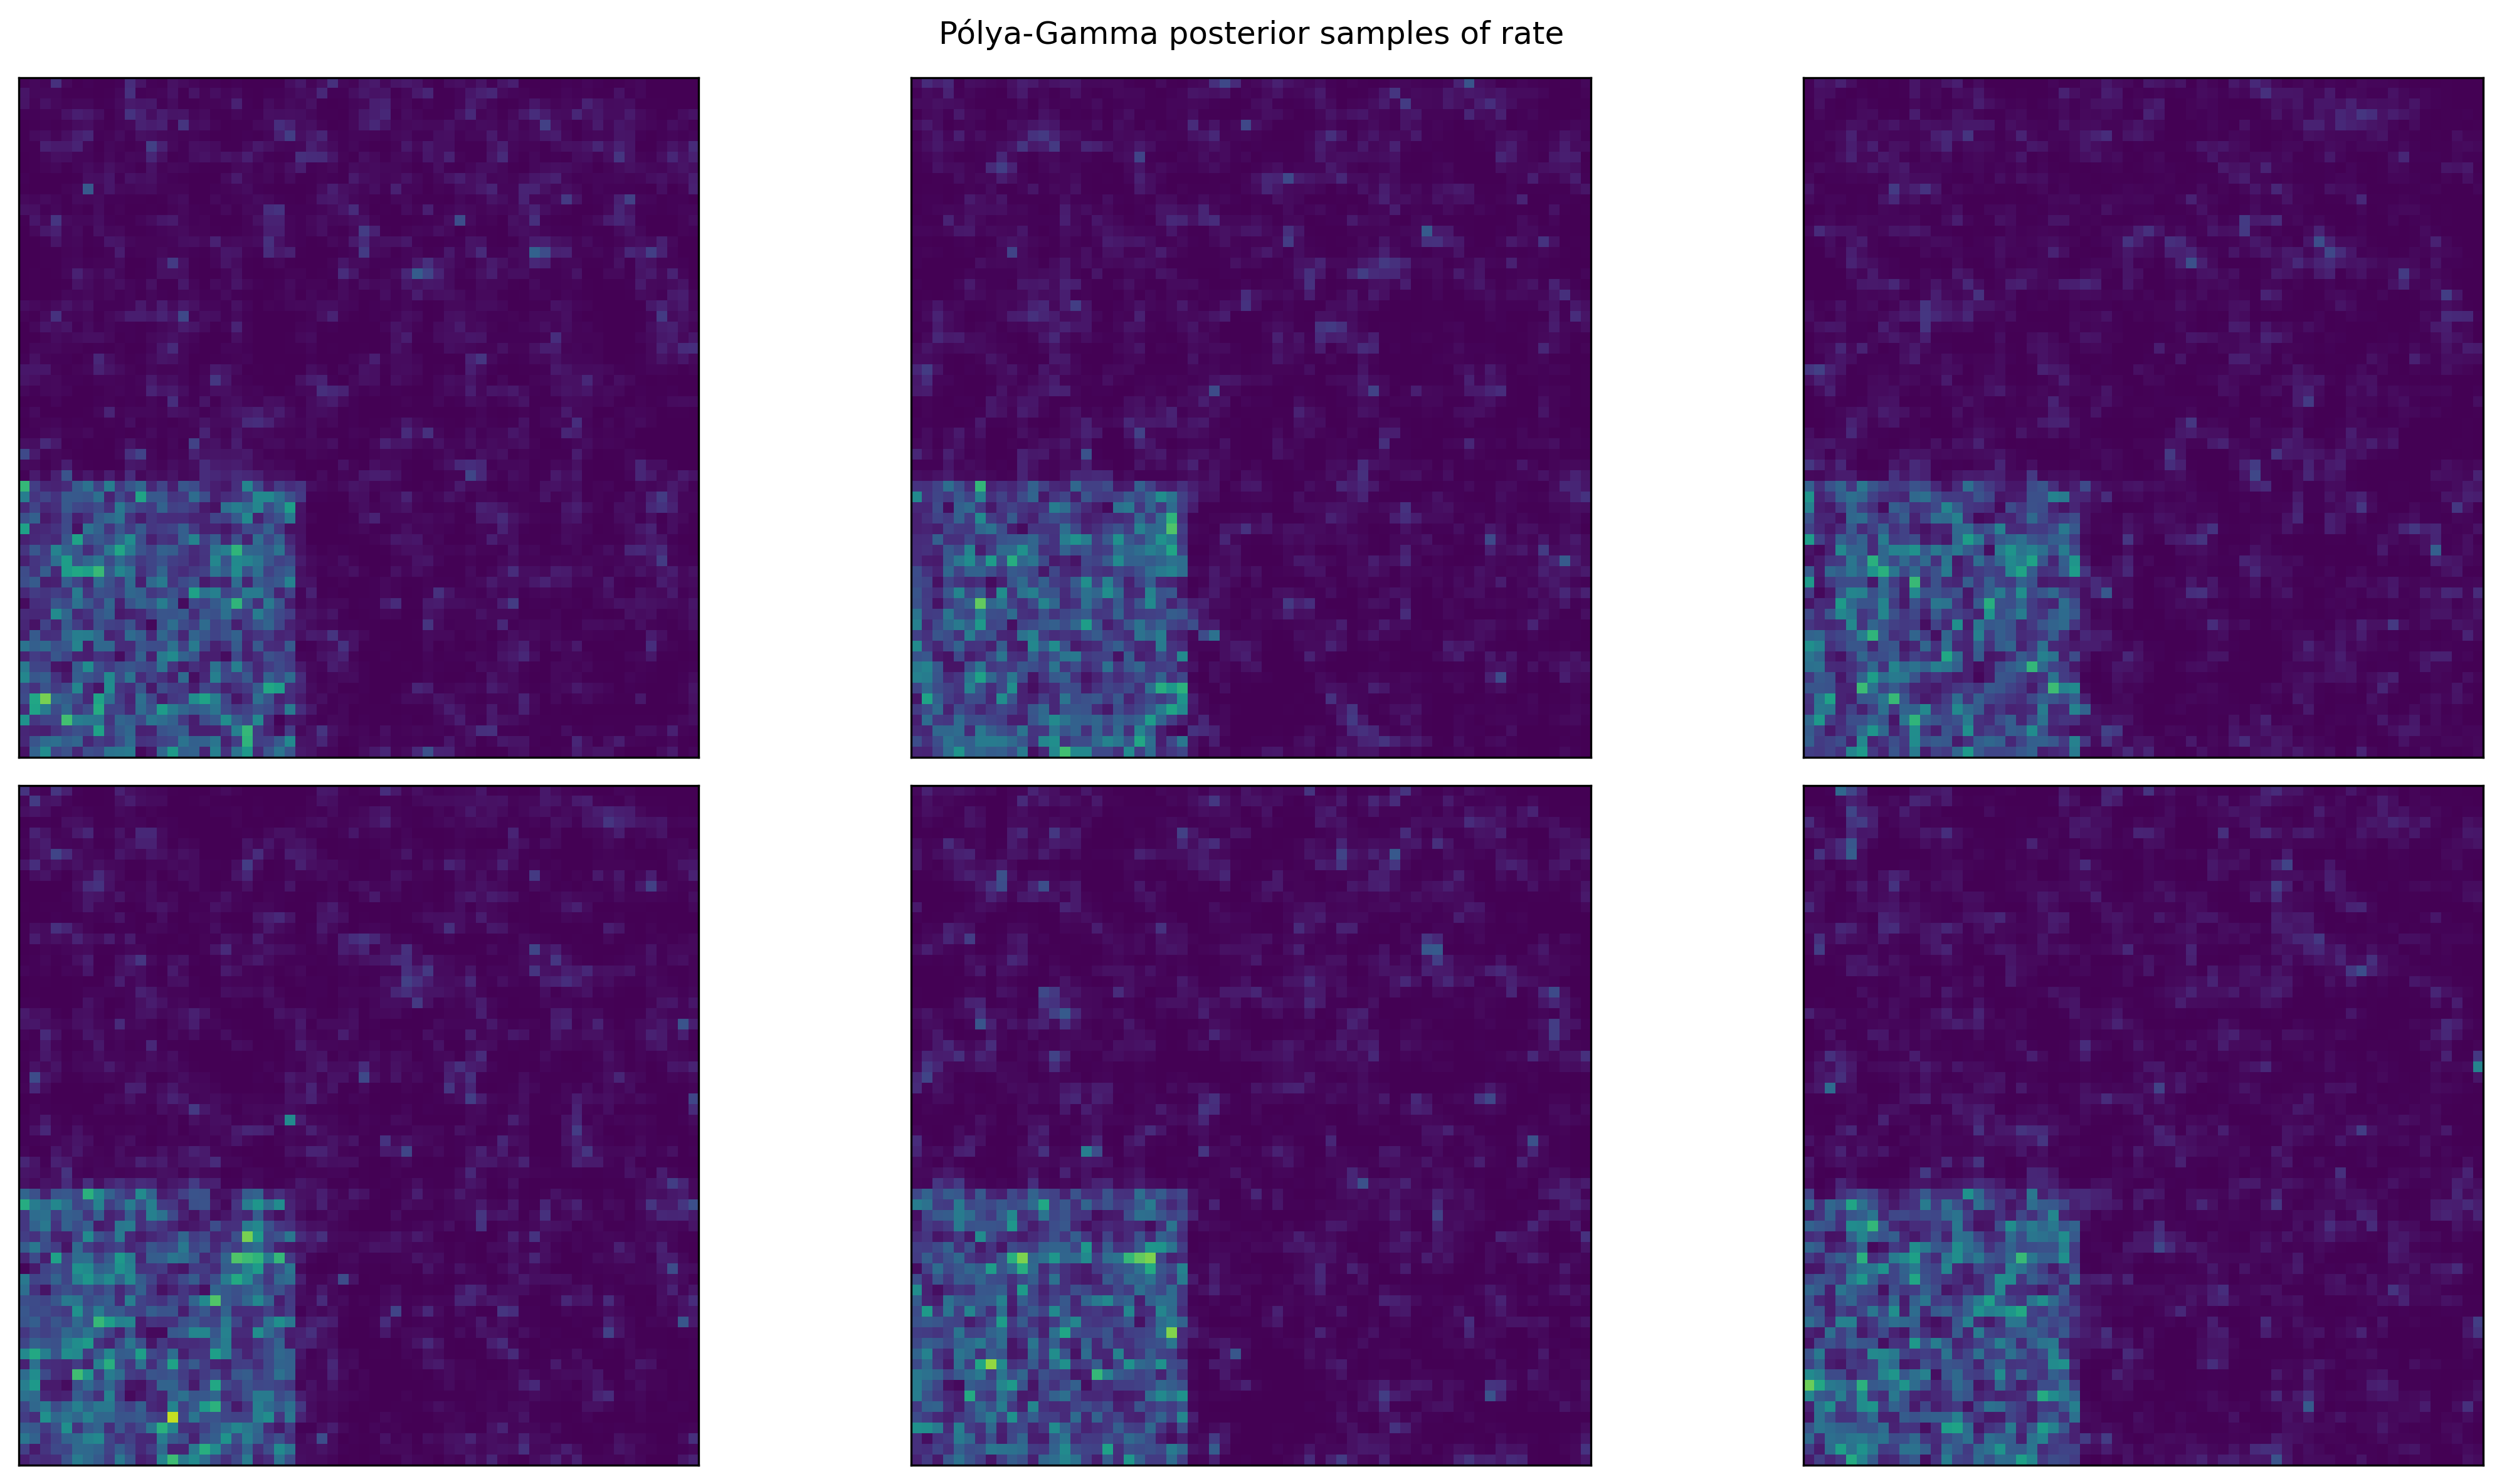
\includegraphics[
    width=\linewidth,
    height=0.66\textheight,
    keepaspectratio
]{figures/synthetic_block_posterior_samples_rho_2_lam_12_var_4.png} 
\end{frame}



%-----------------------------------------------------------


\begin{frame}{Current model configuration}

We model the declustered earthquake counts on a 5 km grid as

$$ n_i \mid f_i \sim \operatorname{Poisson}(\lambda_i),
 \qquad
 \lambda_i = \lambda\,\sigmoid(f_i),
 \qquad
 \sigmoid(f)=\frac{1}{1+e^{-f}}.$$

\medskip
Current parameter choice:
\begin{center}
\begin{tabular}{ll}
\toprule
Grid size & 5 km \\
Catalogue & declustered \\
Spatial scale & $\rho=20$ km \\
Global intensity ceiling & $\lambda=250$ \\
Prior variance parameter & $v^2=4$ \\
Prior latent mean & $\mu_0 = -7.5$ \\
\bottomrule
\end{tabular}
\end{center}

\medskip

\end{frame}

% -----------------------------------------------------------
\begin{frame}{Declustered binned earthquake catalogue}

\begin{columns}[T,onlytextwidth]
\column{0.64\textwidth}
\centering
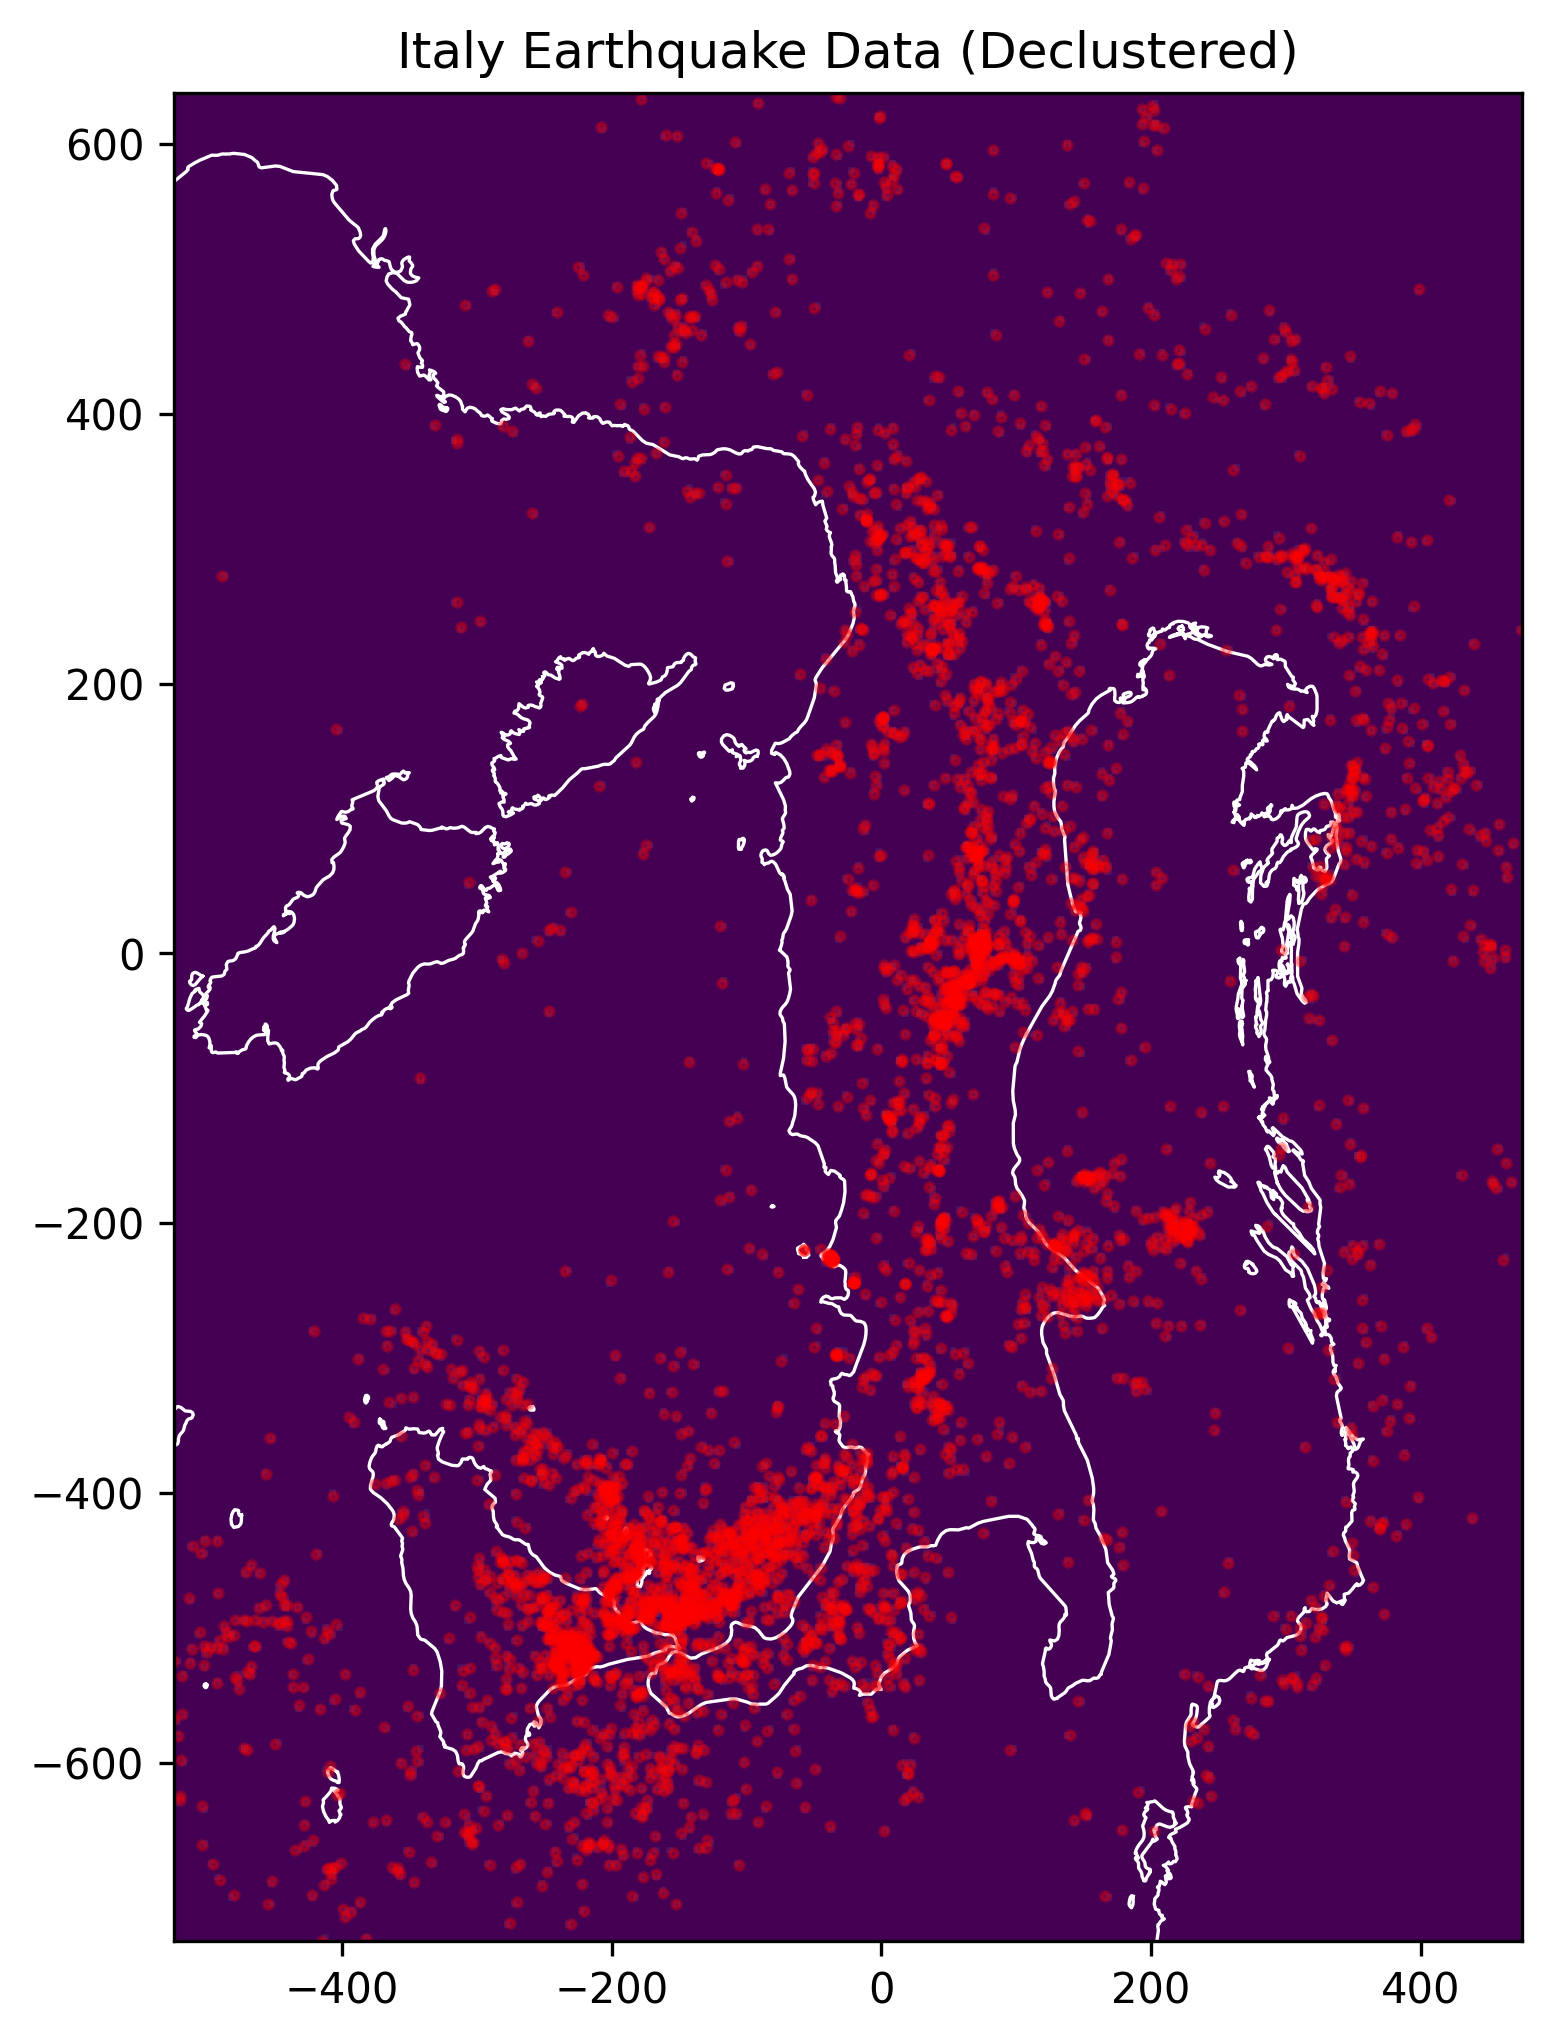
\includegraphics[width=\linewidth,height=0.70\textheight,keepaspectratio]{figures/italy_italy_earthquake_data_bin_5km_declustered.png}

\column{0.34\textwidth}
\small
\begin{tabular}{lr}
\toprule
Statistic & Observed \\
\midrule
Events & 4,943 \\
Grid cells & 54,800 \\
Zero cells & 51,570 \\
One-event cells & 2,385 \\
Cells $\geq 2$ & 845 \\
Cells $\geq 5$ & 105 \\
Cells $\geq 10$ & 16 \\
Cells $\geq 15$ & 5 \\
Maximum count & 23 \\
\bottomrule
\end{tabular}
\end{columns}

\end{frame}

% -----------------------------------------------------------
\begin{frame}{Effect of NND declustering}

\begin{center}
\small

\begin{tabular}{lrr}
\toprule
Statistic & Original catalogue & NND declustered \\
\midrule
Events                 & 11,327 & 4,943 \\
Grid cells             & 54,800 & 54,800 \\
Occupied cells         & 3,518  & 3,230 \\
Zero cells             & 51,282 & 51,570 \\
One-event cells        & 2,319  & 2,385 \\
Cells $\geq 2$         & 1,199  & 845 \\
Cells $\geq 5$         & 298    & 105 \\
Cells $\geq 10$        & 135    & 16 \\
Cells $\geq 15$        & 89     & 5 \\
Maximum count          & 279    & 23 \\
\midrule
Mean count / cell      & 0.2067 & 0.0902 \\
Variance / cell        & 10.1819 & 0.2401 \\
Variance / mean        & 49.26  & 2.66 \\
\bottomrule
\end{tabular}

\end{center}



\end{frame}

% -----------------------------------------------------------


\begin{frame}{Posterior samples}



\centering

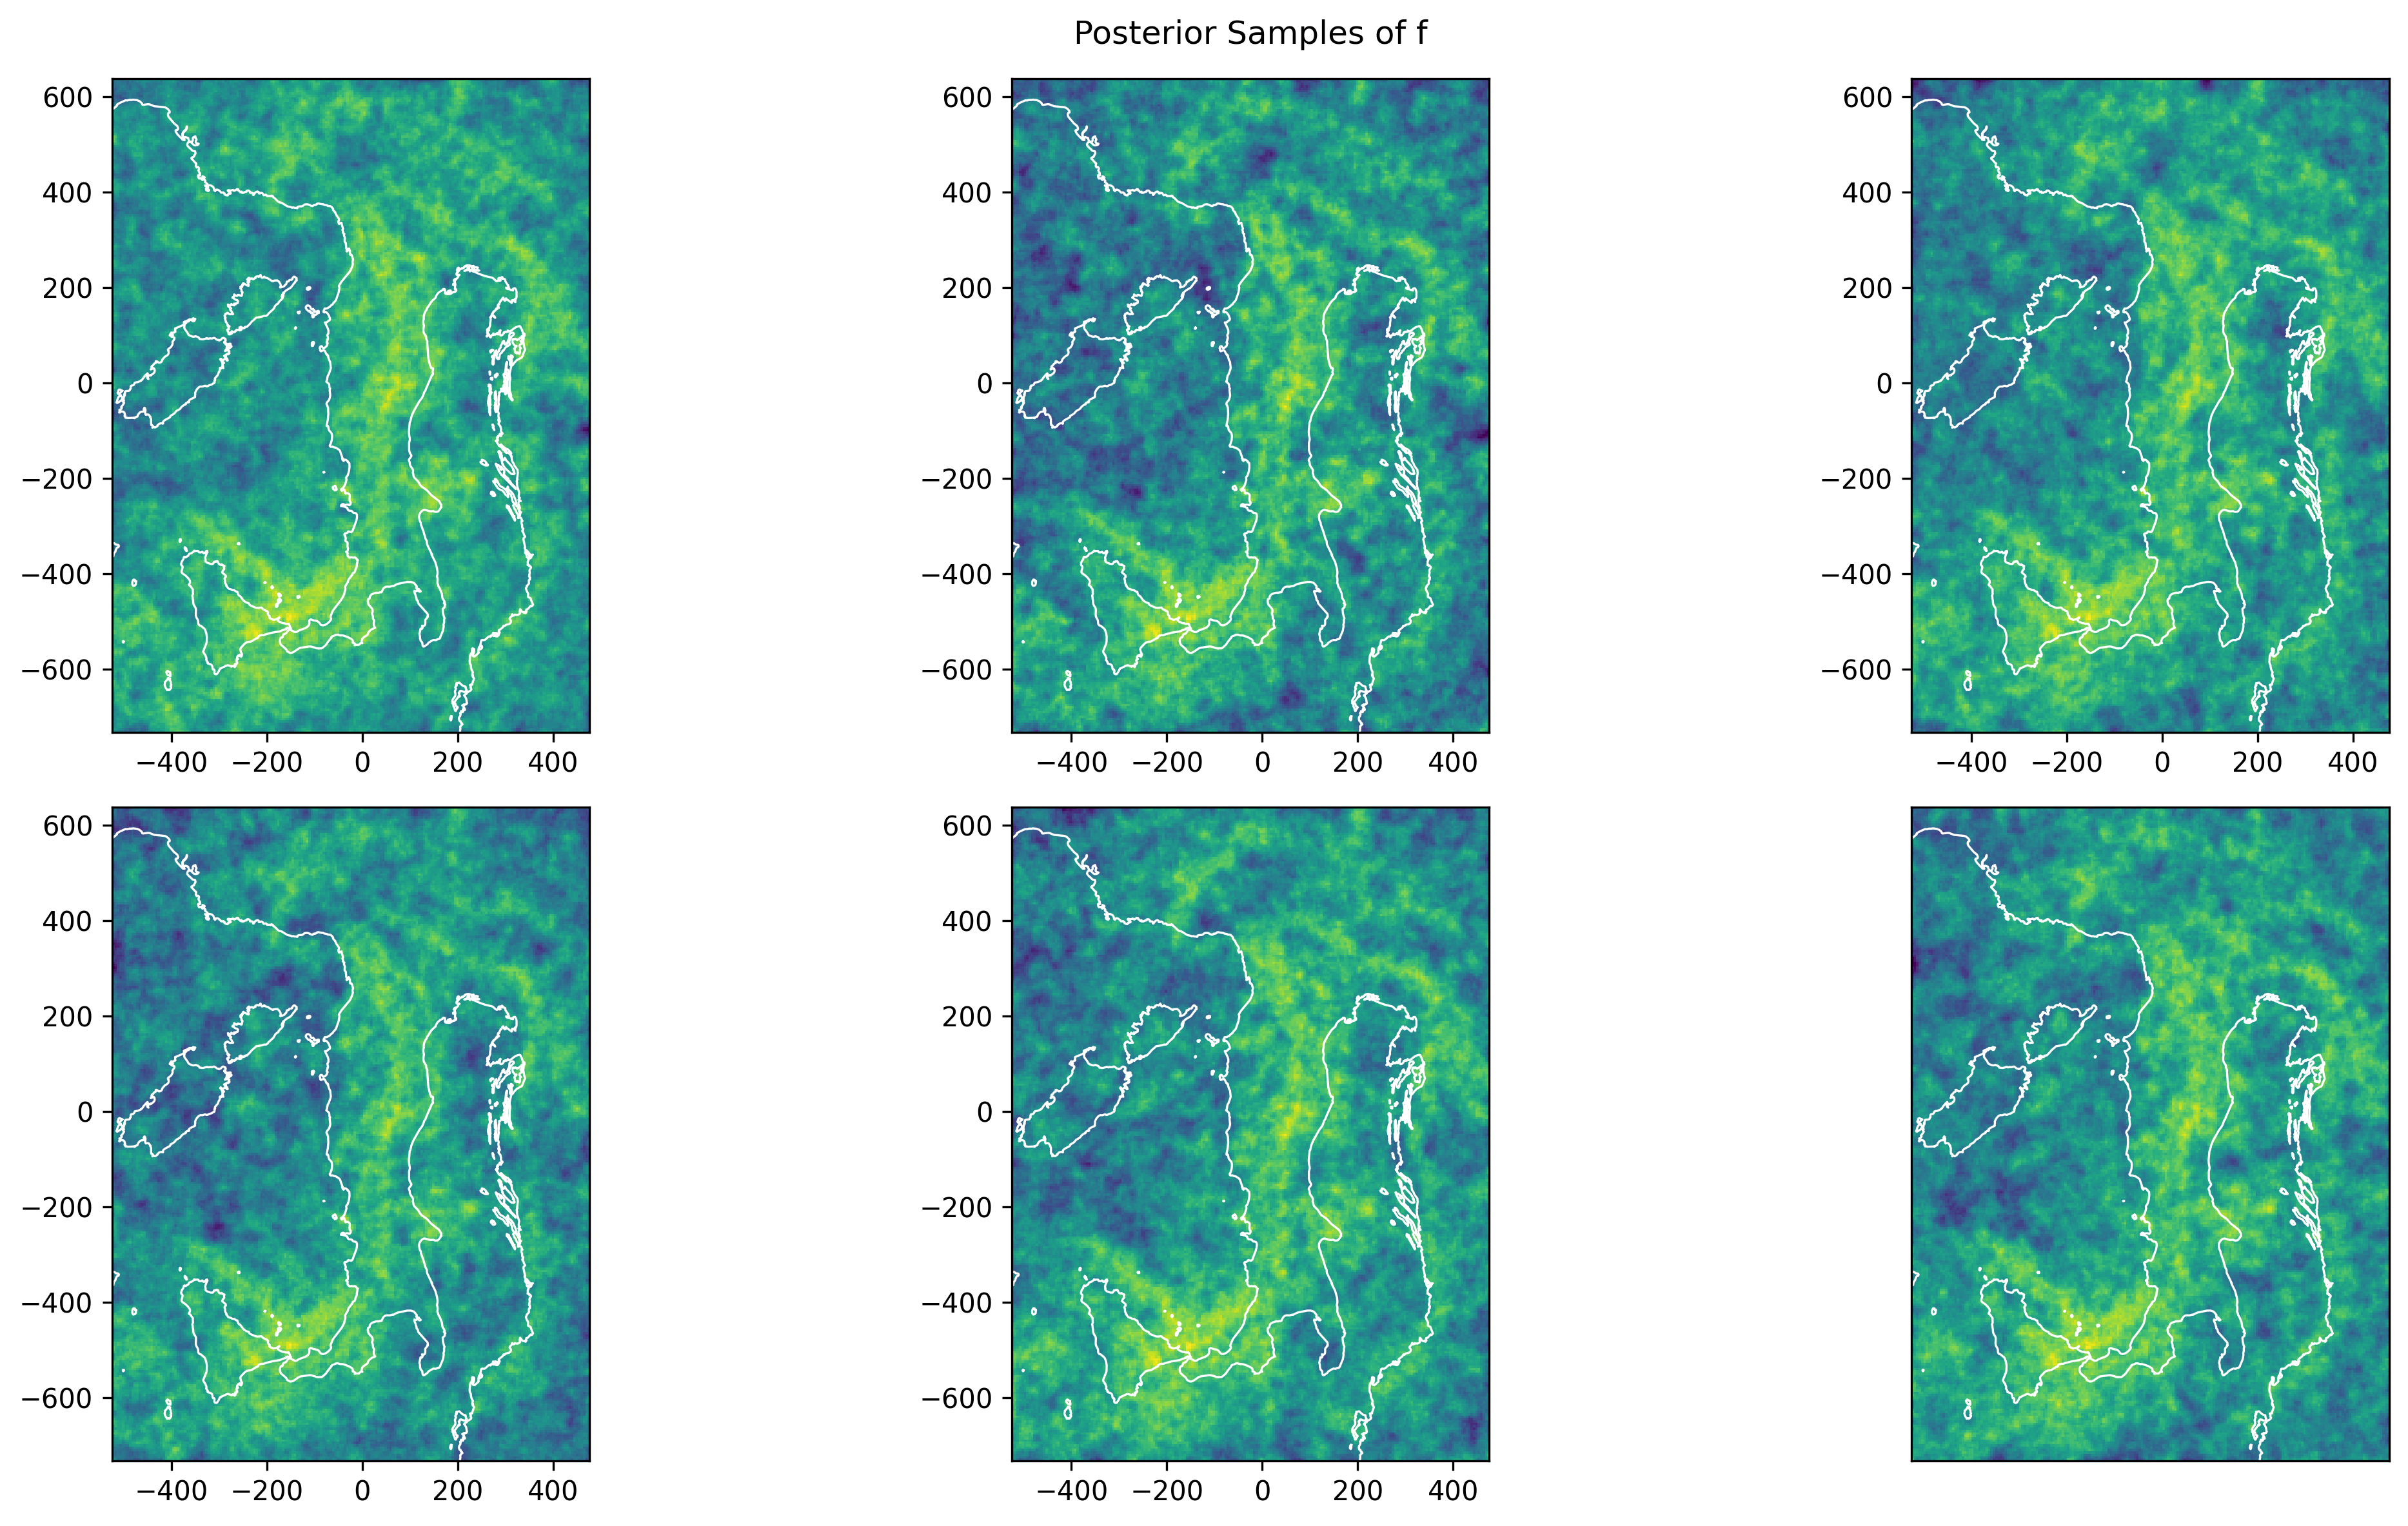
\includegraphics[width=\linewidth,height=0.70\textheight,keepaspectratio]{figures/italy_posterior_samples_bin_5km_declustered.png}



\end{frame}

% -----------------------------------------------------------


\begin{frame}{Latent field: MAP versus posterior mean}

\begin{columns}[T,onlytextwidth]
\column{0.49\textwidth}
\centering
\textbf{MAP estimate}\par\medskip
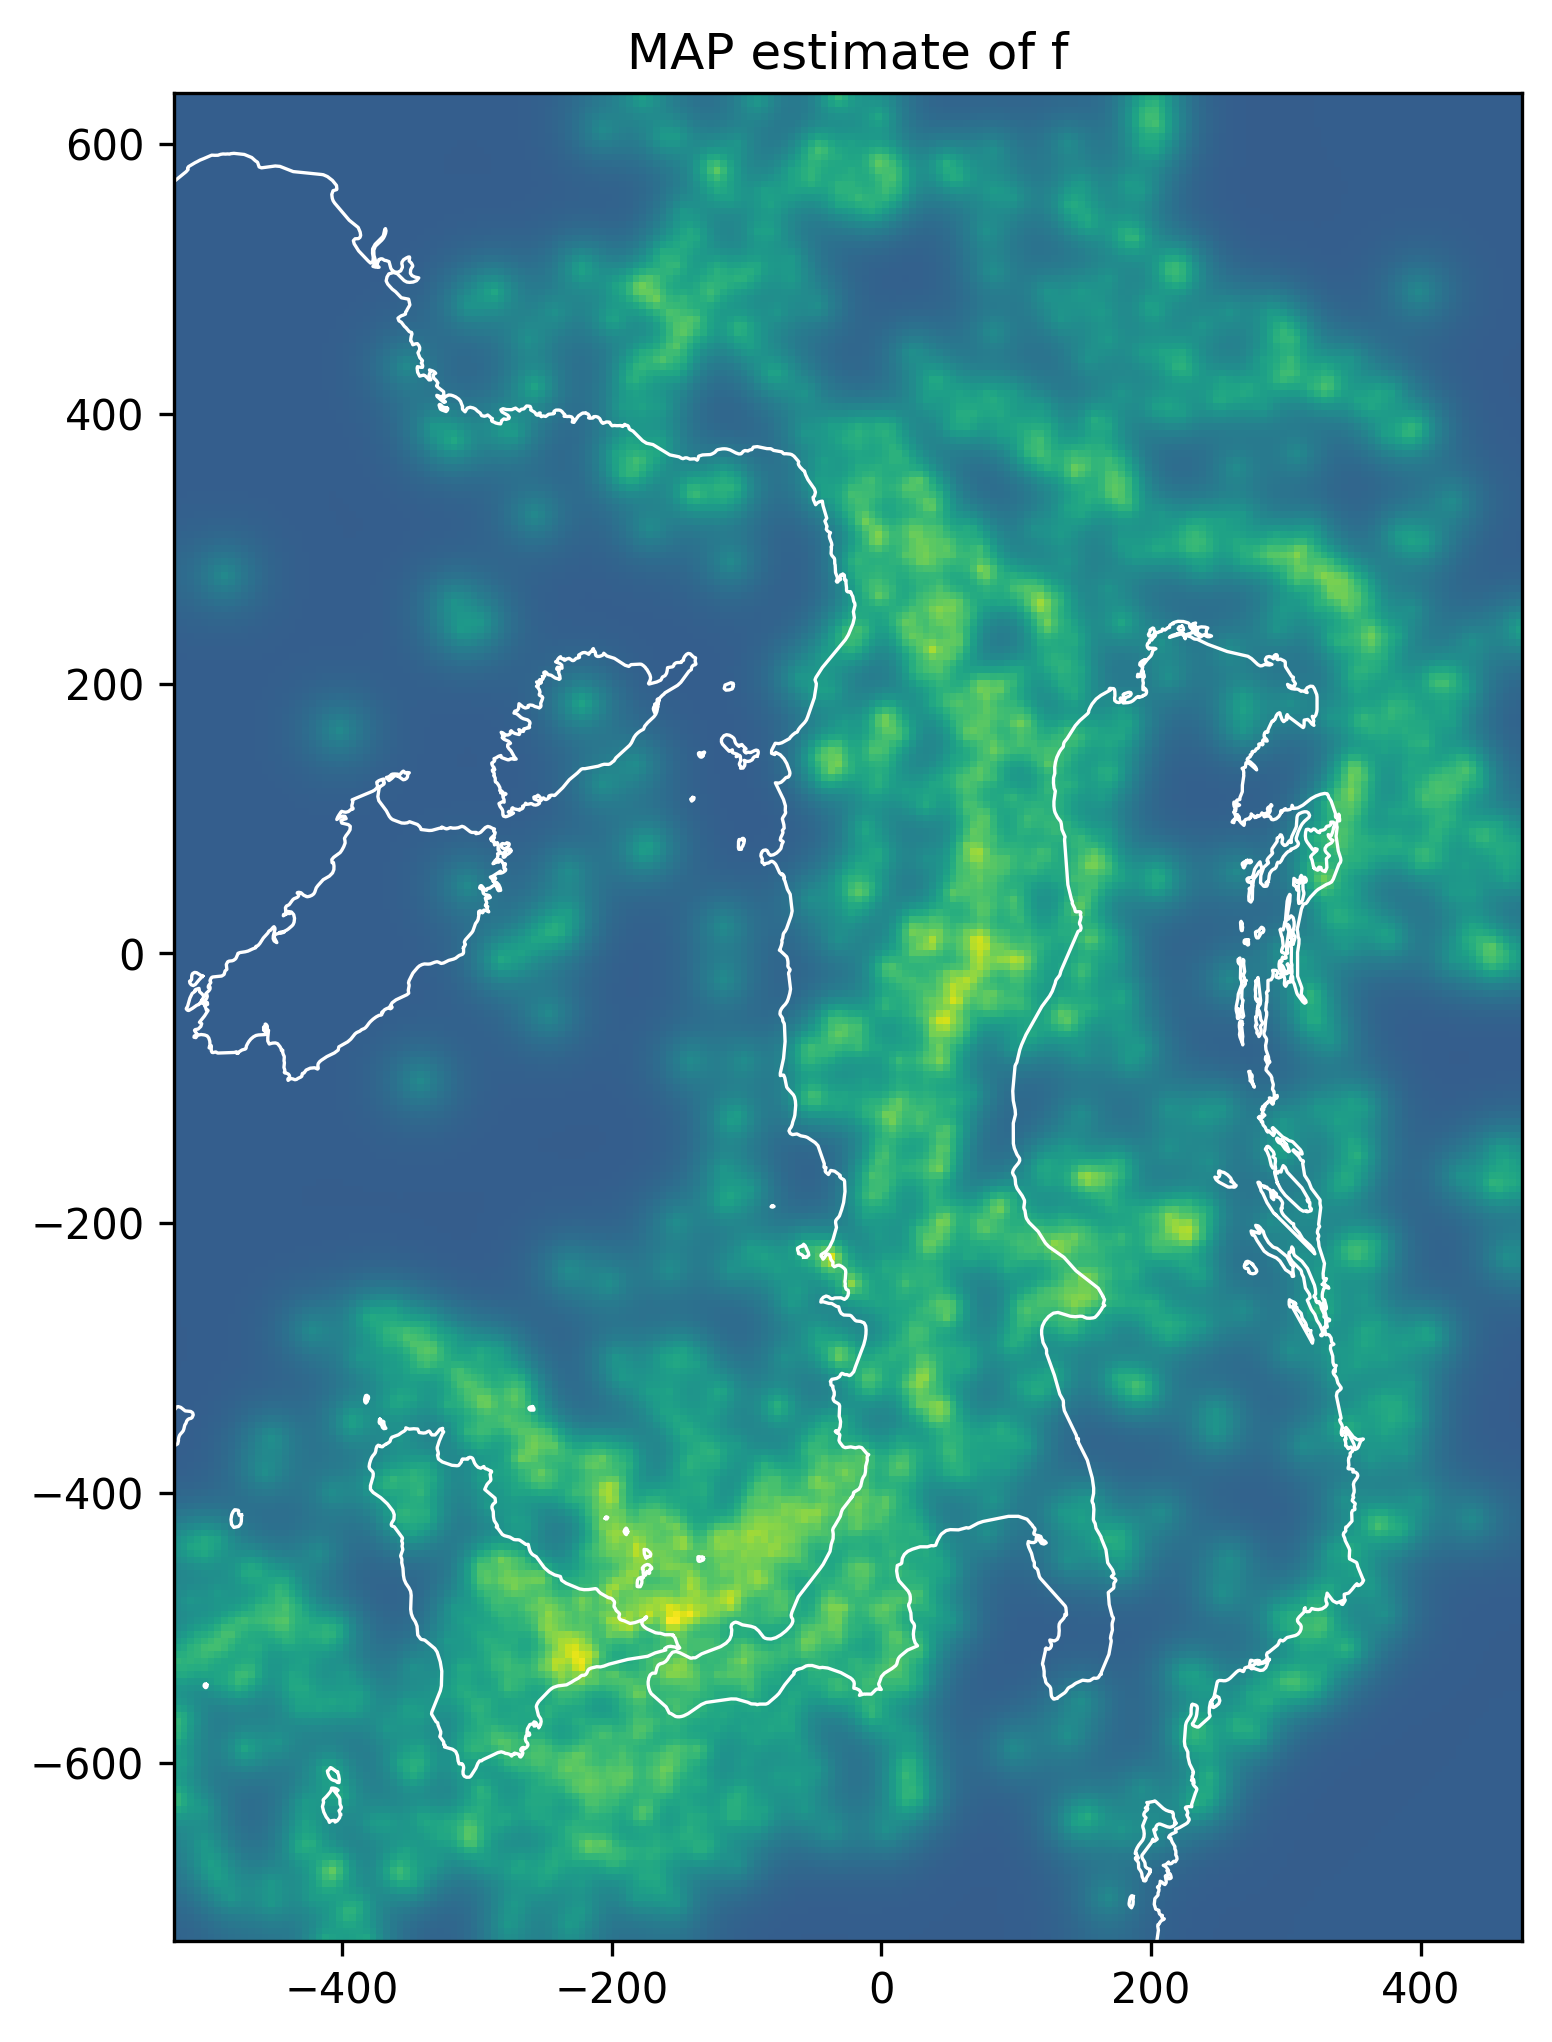
\includegraphics[width=\linewidth,height=0.70\textheight,keepaspectratio]{figures/italy_map_f_bin_5km_declustered.png}

\column{0.49\textwidth}
\centering
\textbf{Posterior mean}\par\medskip

\includegraphics[width=\linewidth,height=0.70\textheight,keepaspectratio]{figures/italy_posterior_mean_f_bin_5km_declustered.png}
\end{columns}

\vspace{-0.2em}
\small

\end{frame}

% -----------------------------------------------------------
\begin{frame}{Posterior mean versus MAP: where do they differ?}

\begin{columns}[T,onlytextwidth]
\column{0.49\textwidth}
\centering
\textbf{Difference in latent field}\par
$\E[f\mid n]-f_{\mathrm{MAP}}$\par\medskip

\includegraphics[width=\linewidth,height=0.70\textheight,keepaspectratio]{figures/italy_difference_f_bin_5km_declustered.png}

\column{0.49\textwidth}
\centering
\textbf{Difference in Poisson rate}\par
$\E[\lambda\mid n]-\lambda(f_{\mathrm{MAP}})$\par\medskip
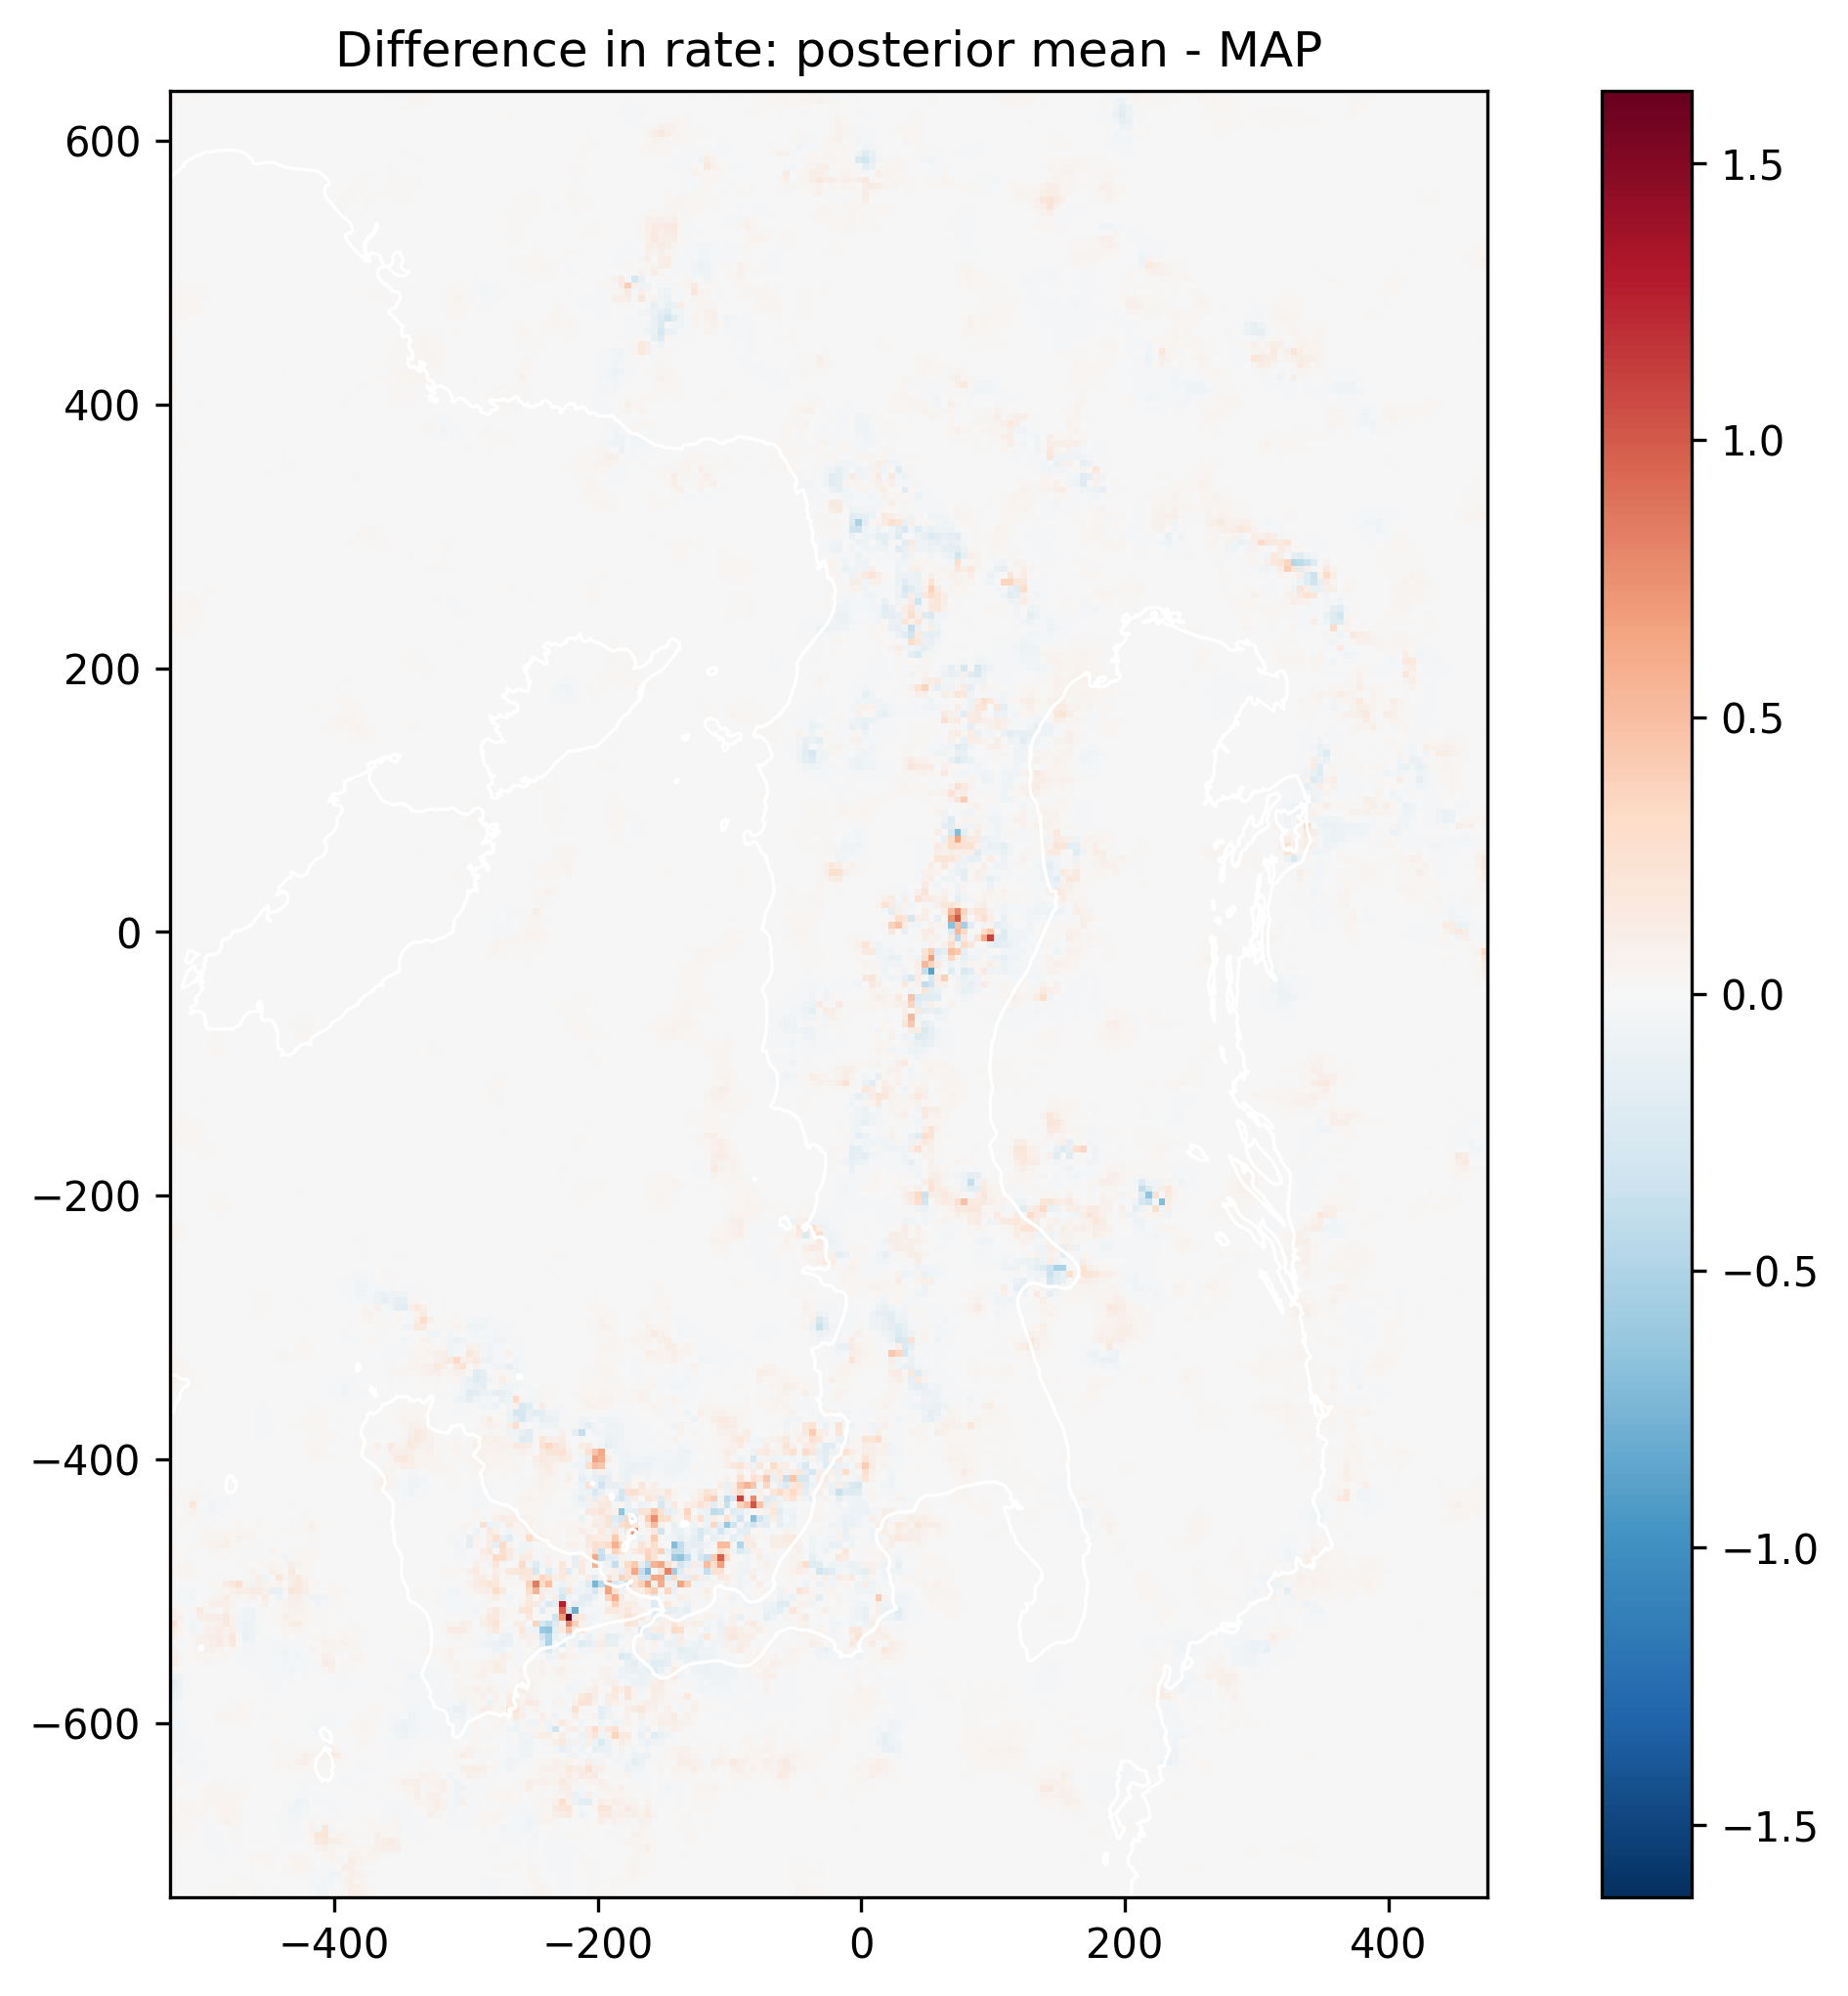
\includegraphics[width=\linewidth,height=0.70\textheight,keepaspectratio]{figures/italy_difference_rate_bin_5km_declustered.png}
\end{columns}

\small


\end{frame}


% -----------------------------------------------------------
\begin{frame}{Posterior sd}

\begin{columns}[T,onlytextwidth]
\column{0.49\textwidth}
\centering


\includegraphics[width=\linewidth,height=0.70\textheight,keepaspectratio]{figures/italy_posterior_sd_f_bin_5km_declustered.png}

\column{0.49\textwidth}
\centering

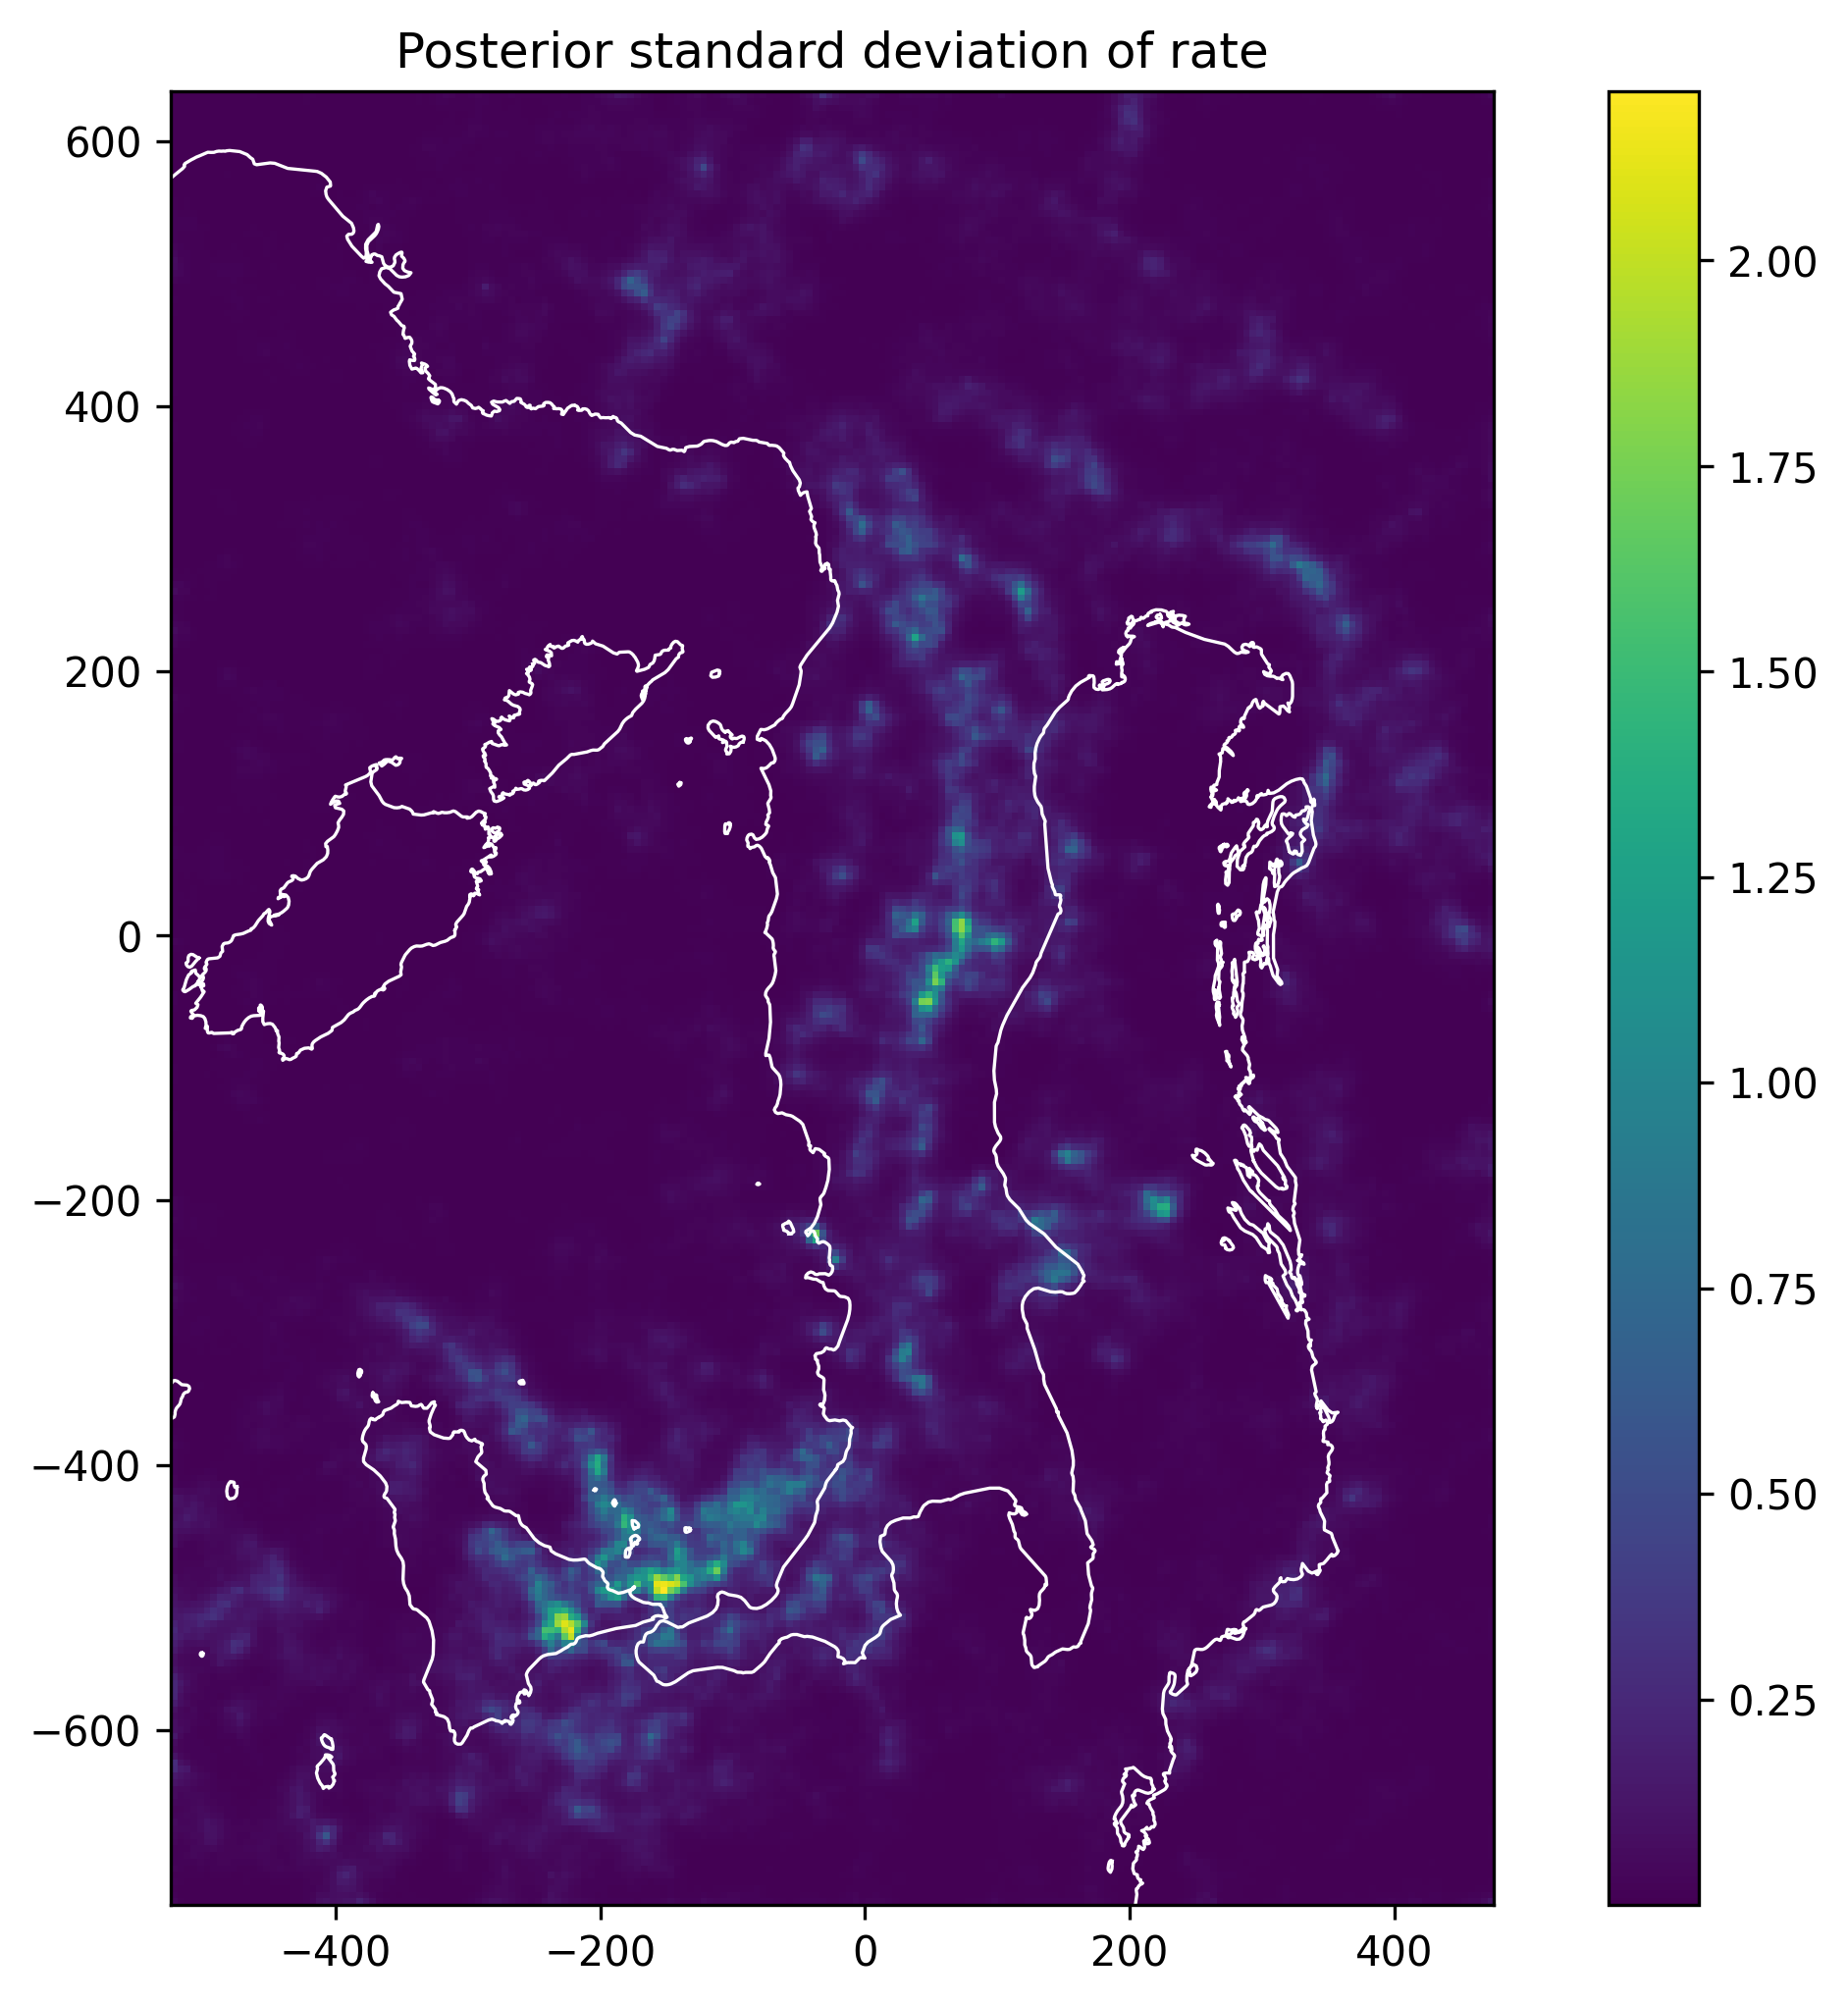
\includegraphics[width=\linewidth,height=0.70\textheight,keepaspectratio]{figures/italy_posterior_sd_rate_bin_5km_declustered.png}
\end{columns}

\small


\end{frame}






\end{document}
